%%%%%%%% ICML 2019 EXAMPLE LATEX SUBMISSION FILE %%%%%%%%%%%%%%%%%

\documentclass{article}

% Recommended, but optional, packages for figures and better typesetting:

\usepackage{caption}
\usepackage{amsthm}
\usepackage{tabularx}
\usepackage{bm}
\usepackage{array}
\usepackage{balance}
\usepackage{amsmath}
\usepackage{amssymb}
\usepackage{multirow}
\usepackage{color}
\usepackage{microtype}
\usepackage{graphicx}
\usepackage{subfigure}
\usepackage{booktabs}
\usepackage{bbm}
\usepackage{multicol}
%\usepackage{algcompatible}


\usepackage[colorlinks,linkcolor=red,citecolor=blue]{hyperref}       % hyperlinks
\usepackage{natbib}
\allowdisplaybreaks

\def\rc{\color {red}}

\DeclareMathOperator*{\Argmax}{Argmax}
\DeclareMathOperator*{\Argmin}{Argmin}

\newcommand{\var}{{\rm var}}
\newcommand{\Tr}{^{\rm T}}
\newcommand{\vtrans}[2]{{#1}^{(#2)}}
\newcommand{\kron}{\otimes}
\newcommand{\schur}[2]{({#1} | {#2})}
\newcommand{\schurdet}[2]{\left| ({#1} | {#2}) \right|}
\newcommand{\had}{\circ}
\newcommand{\diag}{{\rm diag}}
\newcommand{\invdiag}{\diag^{-1}}
\newcommand{\rank}{{\rm rank}}
\newcommand{\expt}[1]{\langle #1 \rangle}
% careful: ``null'' is already a latex command
\newcommand{\nullsp}{{\rm null}}
\newcommand{\tr}{{\rm tr}}
\renewcommand{\vec}{{\rm vec}}
\newcommand{\vech}{{\rm vech}}
\renewcommand{\det}[1]{\left| #1 \right|}
\newcommand{\pdet}[1]{\left| #1 \right|_{+}}
\newcommand{\pinv}[1]{#1^{+}}
\newcommand{\erf}{{\rm erf}}
\newcommand{\hypergeom}[2]{{}_{#1}F_{#2}}
\newcommand{\mcal}[1]{\mathcal{#1}}
\newcommand{\Rcal}{{\mathcal{R}}}
\newcommand{\Acal}{{\mathcal{A}}}
\newcommand{\Ccal}{{\mathcal{C}}}
\newcommand{\Fcal}{{\mathcal{F}}}
% boldface characters
\renewcommand{\a}{{\bf a}}
\renewcommand{\b}{{\bf b}}
\renewcommand{\c}{{\bf c}}
\renewcommand{\d}{{\rm d}}  % for derivatives
\newcommand{\e}{{\bf e}}
\newcommand{\f}{{\bf f}}
\newcommand{\g}{{\bf g}}
\newcommand{\h}{{\bf h}}
\newcommand{\bi}{{\bf i}}
\newcommand{\bj}{{\bf j}}
\newcommand{\bK}{{\bf K}}
\newcommand{\Kcal}{{\mathcal{K}}}
% in Latex2e this must be renewcommand
\renewcommand{\k}{{\bf k}}
\newcommand{\m}{{\bf m}}
\newcommand{\mhat}{{\overline{m}}}
\newcommand{\tm}{{\tilde{m}}}
\newcommand{\n}{{\bf n}}
\renewcommand{\o}{{\bf o}}
\newcommand{\p}{{\bf p}}
\newcommand{\q}{{\bf q}}
\renewcommand{\r}{{\bf r}}
\newcommand{\s}{{\bf s}}
\renewcommand{\t}{{\bf t}}
\renewcommand{\u}{{\bf u}}
\renewcommand{\v}{{\bf v}}
\newcommand{\w}{{\bf w}}
\newcommand{\x}{{\bf x}}
\newcommand{\y}{{\bf y}}
\newcommand{\z}{{\bf z}}
\newcommand{\bl}{{\bf l}}
\newcommand{\A}{{\bf A}}
\newcommand{\B}{{\bf B}}
\newcommand{\C}{{\bf C}}
\newcommand{\D}{{\bf D}}
\newcommand{\Dcal}{\mathcal{D}}
\newcommand{\E}{{\bf E}}
\newcommand{\F}{{\bf F}}
\newcommand{\G}{{\bf G}}
\newcommand{\Gcal}{{\mathcal{G}}}
\renewcommand{\H}{{\bf H}}
\newcommand{\I}{{\bf I}}
\newcommand{\J}{{\bf J}}
\newcommand{\K}{{\bf K}}
\renewcommand{\L}{{\bf L}}
%\newcommand{\Lcal}{{\mathcal{L}}}
\newcommand{\M}{{\bf M}}
\newcommand{\Mcal}{{\mathcal{M}}}
\newcommand{\N}{\mathcal{N}}  % for normal density
%\newcommand{\N}{{\bf N}}
\newcommand{\bupeta}{\boldsymbol{\upeta}}
\renewcommand{\O}{{\bf O}}
\renewcommand{\P}{{\bf P}}
\newcommand{\Q}{{\bf Q}}
\newcommand{\R}{{\bf R}}
\renewcommand{\S}{{\bf S}}
\newcommand{\Scal}{{\mathcal{S}}}
\newcommand{\T}{{\bf T}}
\newcommand{\Tcal}{{\mathcal{T}}}
\newcommand{\U}{{\bf U}}
\newcommand{\Ucal}{{\mathcal{U}}}
\newcommand{\tU}{{\tilde{\U}}}
\newcommand{\tUcal}{{\tilde{\Ucal}}}
\newcommand{\V}{{\bf V}}
\newcommand{\W}{{\bf W}}

\newcommand{\Ocal}[1]{{\mathcal{O}\left( #1  \right)}}
\newcommand{\Omegacal}[1]{{\Omega \left( #1 \right)}}
\newcommand{\Pcal}{{\mathcal{P}}}
\newcommand{\Hcal}{{\mathcal{H}}}
\newcommand{\Wcal}{{\mathcal{W}}}
\newcommand{\X}{{\bf X}}
\newcommand{\Xcal}{{\mathcal{X}}}
\newcommand{\Y}{{\bf Y}}
\newcommand{\Ycal}{{\mathcal{Y}}}
\newcommand{\Z}{{\bf Z}}
\newcommand{\Zcal}{{\mathcal{Z}}}

% this is for latex 2.09
% unfortunately, the result is slanted - use Latex2e instead
%\newcommand{\bfLambda}{\mbox{\boldmath$\Lambda$}}
% this is for Latex2e
\newcommand{\bfLambda}{\boldsymbol{\Lambda}}

% Yuan Qi's boldsymbol
\newcommand{\bsigma}{\boldsymbol{\sigma}}
\newcommand{\balpha}{\boldsymbol{\alpha}}
\newcommand{\bpsi}{\boldsymbol{\psi}}
\newcommand{\bphi}{\boldsymbol{\phi}}
\newcommand{\bbeta}{\boldsymbol{\beta}}
\newcommand{\bepsi}{\boldsymbol{\epsilon}}
\newcommand{\Beta}{\boldsymbol{\eta}}
\newcommand{\btau}{\boldsymbol{\tau}}
\newcommand{\bvarphi}{\boldsymbol{\varphi}}
\newcommand{\bzeta}{\boldsymbol{\zeta}}

\newcommand{\blambda}{\boldsymbol{\lambda}}
\newcommand{\bLambda}{\mathbf{\Lambda}}

\newcommand{\btheta}{\boldsymbol{\theta}}
\newcommand{\bTheta}{\boldsymbol{\Theta}}
\newcommand{\bpi}{\boldsymbol{\pi}}
\newcommand{\bxi}{\boldsymbol{\xi}}
\newcommand{\bSigma}{\boldsymbol{\Sigma}}
\newcommand{\bPi}{\boldsymbol{\Pi}}
\newcommand{\bOmega}{\boldsymbol{\Omega}}
%\newcommand{\bLambda}{\boldsymbol{\Lambda}}

\newcommand{\hatu}{\hat{\bf u}}



\newcommand{\bgamma}{\boldsymbol{\gamma}}
\newcommand{\bGamma}{\boldsymbol{\Gamma}}
\newcommand{\bUpsilon}{\boldsymbol{\Upsilon}}



\newcommand{\bmu}{\boldsymbol{\mu}}
\newcommand{\1}{{\bf 1}}
\newcommand{\0}{{\bf 0}}


\newcommand{\proj}[1]{{\rm proj}\negmedspace\left[#1\right]}
\newcommand{\argmin}{\operatornamewithlimits{argmin}}
\newcommand{\argmax}{\operatornamewithlimits{argmax}}

\newcommand{\dif}{\mathrm{d}}
\newcommand{\lrincir}[1]{\left( #1 \right)}
\newcommand{\abs}[1]{\lvert#1\rvert}
\newcommand{\norm}[1]{\lVert#1\rVert}
\newcommand{\lrnorm}[1]{\left\lVert#1\right\rVert}
\newcommand{\lrangle}[1]{\left\langle#1 \right\rangle}

\newcommand{\ie}{{{i.e.,}}\xspace}
\newcommand{\eg}{{{\em e.g.,}}\xspace}
\newcommand{\EE}{\mathop{\mathbb{E}}}
\newcommand{\RR}{\mathbb{R}}
\newcommand{\sbr}[1]{\left[#1\right]}
\newcommand{\rbr}[1]{\left(#1\right)}
\newcommand{\Lcal}[1]{\mathcal{L}^{#1}_{D_1,D_2}}


\newcommand{\refabove}[2]{\displaystyle_{#1}^{(#2)}}
\newcommand{\refabovecir}[2]{\displaystyle_{#1}^{#2}}



 \newtheorem{Definition}{\bf{Definition}}
 \newtheorem{Theorem}{\bf{Theorem}}
 \newtheorem{reTheorem}[Theorem]{\bf{Theorem}}
 \newtheorem{Lemma}{\bf{Lemma}}
 \newtheorem{reLemma}[Lemma]{\bf{Lemma}}
 \newtheorem{Corollary}{\bf{Corollary}}
 \newtheorem{reCorollary}[Corollary]{\bf{Corollary}}
 \newtheorem{Assumption}{\bf{Assumption}}
 \newtheorem{Proposition}{\bf{Proposition}}
 \newtheorem{Remark}{\bf{Remark}}



 % for professional tables

% hyperref makes hyperlinks in the resulting PDF.
% If your build breaks (sometimes temporarily if a hyperlink spans a page)
% please comment out the following usepackage line and replace
% \usepackage{icml2019} with \usepackage[nohyperref]{icml2019} above.
\usepackage{hyperref}

% Attempt to make hyperref and algorithmic work together better:
\newcommand{\theHalgorithm}{\arabic{algorithm}}

% Use the following line for the initial blind version submitted for review:
\usepackage{icml2019}

% If accepted, instead use the following line for the camera-ready submission:
%\usepackage[accepted]{icml2019}

% The \icmltitle you define below is probably too long as a header.
% Therefore, a short form for the running title is supplied here:
% \icmltitlerunning{Decentralized Online Learning: Exchanging Local Models to Track Dynamics}
\icmltitlerunning{Decentralized Online Learning: Take Benefits from Others' Data without Sharing Your Own to Track Global Dynamics}




\hypersetup{draft}% need to be commit before submitting paper
\begin{document}

\twocolumn[
\icmltitle{Decentralized Online Learning: Take Benefits from Others' Data without Sharing Your Own and Track Global Dynamics}

% It is OKAY to include author information, even for blind
% submissions: the style file will automatically remove it for you
% unless you've provided the [accepted] option to the icml2019
% package.

% List of affiliations: The first argument should be a (short)
% identifier you will use later to specify author affiliations
% Academic affiliations should list Department, University, City, Region, Country
% Industry affiliations should list Company, City, Region, Country

% You can specify symbols, otherwise they are numbered in order.
% Ideally, you should not use this facility. Affiliations will be numbered
% in order of appearance and this is the preferred way.
\icmlsetsymbol{equal}{*}

\begin{icmlauthorlist}
\icmlauthor{Aeiau Zzzz}{equal,to}
\icmlauthor{Bauiu C.~Yyyy}{equal,to,goo}
\icmlauthor{Cieua Vvvvv}{goo}
\icmlauthor{Iaesut Saoeu}{ed}
\icmlauthor{Fiuea Rrrr}{to}
\icmlauthor{Tateu H.~Yasehe}{ed,to,goo}
\icmlauthor{Aaoeu Iasoh}{goo}
\icmlauthor{Buiui Eueu}{ed}
\icmlauthor{Aeuia Zzzz}{ed}
\icmlauthor{Bieea C.~Yyyy}{to,goo}
\icmlauthor{Teoau Xxxx}{ed}
\icmlauthor{Eee Pppp}{ed}
\end{icmlauthorlist}

\icmlaffiliation{to}{Department of Computation, University of Torontoland, Torontoland, Canada}
\icmlaffiliation{goo}{Googol ShallowMind, New London, Michigan, USA}
\icmlaffiliation{ed}{School of Computation, University of Edenborrow, Edenborrow, United Kingdom}

\icmlcorrespondingauthor{Cieua Vvvvv}{c.vvvvv@googol.com}
\icmlcorrespondingauthor{Eee Pppp}{ep@eden.co.uk}

% You may provide any keywords that you
% find helpful for describing your paper; these are used to populate
% the "keywords" metadata in the PDF but will not be shown in the document
\icmlkeywords{Machine Learning, ICML}

\vskip 0.3in
]

% this must go after the closing bracket ] following \twocolumn[ ...

% This command actually creates the footnote in the first column
% listing the affiliations and the copyright notice.
% The command takes one argument, which is text to display at the start of the footnote.
% The \icmlEqualContribution command is standard text for equal contribution.
% Remove it (just {}) if you do not need this facility.

%\printAffiliationsAndNotice{}  % leave blank if no need to mention equal contribution
\printAffiliationsAndNotice{\icmlEqualContribution} % otherwise use the standard text.


\begin{abstract}
Decentralized Online Learning (Online learning in decentralized networks) attracts more and more attention, since it is believed that Decentralized Online Learning can help the data providers cooperatively better solve their online problems without sharing their private data to a third party or other providers.
Typically, the cooperation is achieved by letting the data providers exchange their models between neighbors, e.g., recommendation model. However, the best regret bound for a decentralized online learning algorithm is $\Ocal{n\sqrt{T}}$, where $n$ is the number of nodes (or users) and $T$ is the number of iterations. This is clearly insignificant since this bound can be achieved \emph{without} any communication in the networks. {\rc This reminds us to ask a fundamental question: \emph{Can people really get benefit from the decentralized online learning by exchanging information?}
In this paper, we studied when and why the communication can help the decentralized online learning to reduce the regret.
Specifically, each loss function is characterized by two components: the adversarial component and the random component.
%we assume each loss function consists of an adversarial loss and a stochastic loss.
Under this characterization, we show that decentralized online gradient (DOG) enjoys a regret bound  $\Ocal{n\sqrt{T}G + \sqrt{nT}\sigma}$, where $G$ measures the magnitude of the adversarial component in the private data (or equivalently the local loss function) and $\sigma$ measures the randomness within the private data. This regret suggests that people can get benefits from the randomness in the private data by exchanging private information. Another important contribution of this paper is to consider the dynamic regret -- a more practical regret to track users' interest dynamics.}
%For this bound, the $\Ocal{n\sqrt{T}}$ is due to the adversary loss, while the $\Ocal{\sqrt{nT}\sigma}$ is due to the stochastic loss, which indicates that.
%the online stochastic setting is more suitable for decentralized online learning.
Empirical studies are also conducted to validate our analysis. 

%In addition, to consider more practical scenario we allow users' interest changing over time (it means that the optimal model changes over time), unlike most online works which assume that the optimal prediction model is constant. 
%This study indicates the possibility of a new framework of data service: all users can take benefit from their private data without sharing them.
\end{abstract}


\section{Introduction}
\label{sect_introduction}
Decentralized Online Learning (or, online learning in decentralized networks) receives extensive attentions in recent years~\citep{8015179Shahram,Kamp:2014:CDO,Koppel-8352032,Zhang2018,pmlr-v70-zhang17g,Xu2015,tcns-7353155,cdc-7798923,acc-7172037,tcns-7479495,Benczur:2018ww,tkde-6311406}. 
It assumes that computational nodes in a network can communicate between neighbors to minimize an overall cumulative regret.
Each computational node, which could be a user in practice, will receive a stream of online losses that are usually determined by a sequence of examples that arrive sequentially. 
Formally, we can denote $f_{i,t}$  as the loss received by the $i$-th computational node among the networks at the $t$-th iteration. 
The goal of decentralized online learning usually is to minimize its static regret, which is defined as the difference between the cumulative loss (the sum of all the online loss over all the nodes and steps ) suffered by the learning algorithm and that of the best model which can observe all the loss functions beforehand. 

Decentralized online learning attracts more and more attentions recently, mainly because it is believed by the community that it enjoys the following advantages for real-world large-scale applications:
\begin{itemize}
\item ({\bf Utilize all computational resource}) It can utilize the computational resource (of edging devices) by avoiding collecting all the loss functions (or equivalently data) to one central node and put all computational burden on a single node. %which will result in heavy communication cost for the network and extremely high computational cost for the node.
\item ({\bf Protect data privacy}) It can help many data providers collaborate to better minimize their cumulative loss, while at the same time protecting the data privacy as much as possible. 
\end{itemize}
However, the current theoretical study does not explain why people need to use decentralized online learning, since the currently best regret result for decentralized online learning ($\Ocal{n\sqrt{T}}$) for convex loss functions~\citep{6760092,tkde-6311406}) is equal to the overall regret if each node (user) only runs local online gradient without any communication with others\footnote{$n$ is the number of nodes or users and $T$ is the total number of iterations. The regret of an online algorithm is $\Ocal{\sqrt{T}}$ for convex loss functions~\citep{Hazan2016Introduction,ShalevShwartz:2012dz}. Therefore, the overall regret is $n\sqrt{T}$ if all users do not communicate.}. 


% Theoretically, the best static regret bound of a decentralized online learning algorithm is $\Ocal{n\sqrt{T}}$ for convex loss functions as far as we know~\citep{6760092,tkde-6311406}, where $n$ is the number computational nodes and $T$ is the number of iterations. However, this bound can also be achieved by running the online learning algorithm independently on each computational node (or user) \emph{without} any communication, since the regret of an online algorithm is $\Ocal{\sqrt{T}}$ for convex loss functions~\citep{Hazan2016Introduction,ShalevShwartz:2012dz}. 

Therefore, this reminds us to ask a fundamental question: 

\emph{Can people really get benefit with respect to the regret from the decentralized online learning by exchanging information?}

In this paper, we mainly study when can the communication really help decentralized online learning to minimize its regret. Specifically, we distinguish two components in the loss function $f_{i,t}$: the adversary component and the random compoent. Then we prove that decentralized online gradient can achieve a static regret bound of $\Ocal{n\sqrt{T} + \sqrt{nT}\sigma}$ ($\sigma$ measures the randomness of the private data), where the first component of the bound is due to the adversary loss while the second component is due to the stochastic loss.
Moreover, if a dynamic sequence of models with a budget $M$ is used as the reference points, the dynamic regret of the decentralized online gradient is $\Ocal{n\sqrt{TM} + \sqrt{nTM}\sigma}$. {\rc To Peilin: say something to motivate why we want to use dynamic regret.} This shows the communication can help to minimize the stochastic losses, rather than the adversary losses. This result is further verified empirically by extensive experiments on several real datasets.

\paragraph{Notations and definitions}
In the paper, we make the following notations.
\begin{itemize}
\item For any $i\in[n]$ and $t\in[T]$, the random variable $\xi_{i,t}$ is subject to a distribution $D_{i,t}$, that is, $\xi_{i,t} \sim D_{i,t}$. Besides, a set of random variables $\Xi_{n,T}$ and the corresponding set of distributions are defined by
\begin{align}
\nonumber
\Xi_{n,T} = & \{ \xi_{i,t} \}_{1\le i \le n, 1 \le t \le T}, \\
\Dcal_{n,T} = & \{ D_{i,t} \}_{1 \le t \le T},
\end{align} respectively. For math brevity, we use the notation $\Xi_{n,T} \sim \Dcal_{n,T}$ to represent that $\xi_{i,t} \sim D_{i,t}$ holds for any $i\in[n]$ and $t\in[T]$. $\EE$ represents mathematical expectation.
\item For a decentralized network, we use $\W \in\RR^{n\times n}$ to represent its confusion matrix. It is a symmetric doublely stochastic matrix, which implies that every element of $\W$ is non-negative, $\W \1 = \1$, and $\1\Tr\W  = \1\Tr$. We use $\{\lambda_i\}_{i=1}^n$ with $\lambda_1 \ge \lambda_2 \ge \cdots \ge \lambda_n$ to represent its eigenvalues. Note that $\lambda_1 = 1$.
\item $\nabla$ represents gradient operator. $\lrnorm{\cdot}$ represents the $\ell_2$ norm in default.
\item $\lesssim$ represents ``less than equal up to a constant factor".
\item $\Acal$ represents the set of all online algorithms.
\item $\1$ and $\0$ represent all the elements of a vector is $1$ and $0$, respectively.
\end{itemize} 
    











\section{Related work}
\label{sect_related_work}
Online learning has been studied for decades of years. The static regret of a sequential online convex optimization method can achieve $\Ocal{\sqrt{T}}$ and $\Ocal{\log T}$ bounds for convex and strongly convex loss functions, respectively \citep{Hazan2016Introduction,ShalevShwartz:2012dz,introduction-online-optimization}. Recently, both the decentralized online learing and the dynamic regret have drawn much attention due to their wide existence in the practical big data scenarios.
\subsection{Decentralized online learning}
Online learning in a decentralized network has been studied in \citep{8015179Shahram,Kamp:2014:CDO,Koppel-8352032,Zhang2018,pmlr-v70-zhang17g,Xu2015,tcns-7353155,cdc-7798923,acc-7172037,tcns-7479495,Benczur:2018ww,tkde-6311406}.  \citet{8015179Shahram} studies decentralized online mirror descent, and provides $\Ocal{n\sqrt{nTM}}$ dynamic regret. Here, $n$, $T$, and $M$ represent the number of nodes in the newtork, the number of iterations, and the budget of dynamics, respectively.  When the Bregman divergence in the decentralized online mirror descent is chosen appropriately, the decentralized online mirror descent becomes identical to the decentralized online gradient descent. Using the same definition of dynamic regret (defined in \eqref{equa_definition_previous_regret}), our method obtains $\Ocal{n\sqrt{TM}}$ dynamic regret for a decentralized online gradient descent, which is better than $\Ocal{n\sqrt{nTM}}$ in \citet{8015179Shahram}. The improvement of our bound benefits from a better bound of network error (see Lemma \ref{Lemma_x_variance_norm_square}). \citet{Kamp:2014:CDO} studies decentralized online prediction, and presents $\Ocal{\sqrt{nT}}$ static regret.  It assumes that all data, used to yielded the loss, is generated from an unknown distribution. The strong assumption is not practical in the dynamic environment, and thus limits its novelity for a general online learning task. 
Additionally, many decentralized online optimization methods are proposed, for example, decentralized online multi-task learning \citep{Zhang2018}, decentralized online ADMM \citep{Xu2015}, decentralized online gradient descent \citep{tcns-7353155}, decentralized continuous-time online saddle-point method \citep{cdc-7798923}, decentralized online  Nesterov's primal-dual method \citep{acc-7172037,tcns-7479495}, and online distributed dual averaging\citep{6760092}. Those previous methods are proved to yield $\Ocal{\sqrt{T}}$ static regret, which do not have theoretical guarantee of regret in the dynamic environment.   Besides,  \citet{tkde-6311406} provides necessary and sufficient conditions to preserve privacy for decentralized online learning methods, which  is interesting to extend our method to be privacy-preserving in the future work.


\subsection{Dynamic regret}

Dynamic regret has been widely studied for decades of years \citep{Zinkevich:2003,Hall:2015ct,Hall:2013vr,Jadbabaie:2015wg,Yang:2016ud,Bedi:2018te,Zhang:2016wl,Mokhtari:2016jz,Zhang:2018tu,Gyorgy:2016,NIPS2016_6536,Zhao:2018wx}.   For any online algorithm $A\in\Acal$, \citet{Zinkevich:2003} first define the dynamic regret by $\sum_{t=1}^T \lrincir{ f_{t}(\x_{t}) - f_{t}(\x_t^\ast) }$ subject to $\sum_{t=1}^{T-1} \lrnorm{\x_{t+1}^\ast - \x_t^\ast} \le M$. They then propose an online gradient descent method, which yields $\Ocal{\sqrt{TM}+\sqrt{T}}$ regret by choosing an appropriate learning rate. The following researches achieve the sublinear dynamic regret, but extend the analysis of regret by using different reference points. For example, \citet{Hall:2015ct,Hall:2013vr} choose the reference points $\{\x_t^{\ast}\}_{t=1}^T$ satisfying $\sum_{t=1}^{T-1} \lrnorm{\x_{t+1}^\ast - \Phi(\x_t^\ast)} \le M$, where $\Phi(\x_t^\ast)$ is the predictive optimal modelmodel. When the function $\Phi$ predicts accurately, a small $M$ is enough to bound the dynamics. The dynamic regret is thus effectively decreased. \citet{Jadbabaie:2015wg,Yang:2016ud,Bedi:2018te,Zhang:2016wl,Mokhtari:2016jz,Zhang:2018tu} chooses the reference points $\{\y_t^{\ast}\}_{t=1}^T$ with $\y_t^{\ast} = \argmin_{\z\in\Xcal} f_t(\z)$, where $f_t$ is the loss function at the $t$-th iteration. \citet{Gyorgy:2016} provides a new analysis framework, which achieves $\Ocal{\sqrt{TM}}$ dynamic regret\footnote{\citet{Gyorgy:2016} uses the notation of ``shifting regret" instead of ``dynamic regret". In the paper, we keep using ``dynamic regret" as used in most previous literatures. } for any given reference points. Besides, \citet{Zhao:2018wx} presents that the lower bound of the dynamic regret is $\Omega\lrincir{\sqrt{TM}}$. The previous definition of the regret  is a special case of our new definition. Our analysis achieves the tight regret $\Ocal{\sqrt{TM}}$ for the special case of $n=1$ and $\sigma = 0$. 

In some literatures, the regret in a dynamic environment is measured by the number of changes of a reference point over time. It is usually denoted by shifting regret or tracking regret \citep{Herbster1998,Gyorgy:2005wo,Gyorgy:2012wa,Gyorgy:2016,Mourtada:2017vn,JMLR:v17:13-533,NIPS2016_6536,cesabianchi:hal,pmlr-v84-mohri18a,pmlr-v54-jun17a}. Both the shifting regret and the tracking regret can be considered as a variation of the dynamic regret, and is usually studied in the setting of ``learning with expert advice". But, the dynamic regret is usually studied in a general setting of online learning.





\section{Problem formulation}

Suppose that there are $n$ users. Each user maintains a local predictive model, and only talk to his/her neighbors. Let $\x_{i, t}$ denote the local model for user $i$ at iteration $t$. In iteration $t$ user $i$ applies the local model $\x_{i,t}$ to a function $f_{i,t}(\cdot; \xi_{i,t})$ and receives the loss $f_{i,t}(\cdot; \xi_{i,t})$. $\xi_{i,t}$'s are independent to each other in terms of $i$ and $t$, charactering the \emph{stochastic} component in the function $f_{i,t}(\cdot; \xi_{i,t})$, while the subscripts $i$ and $t$ of $f$ indicate the \emph{adversarial} component, for example, the user's profile, location, local time, and etc. {\rc \textbf{From Yawei:} The stochastic component in the function is usually caused by the potential realtion among local models. For example, users' perference to music may be impacted by a popular trend in the Internet at the same time. } 






\paragraph{Communication network.} Users do not want to share the information to others, and can only share their private models to their neighbors (or friends). The communication network can be denoted by an undirected graph $\Gcal=(\text{nodes:} [n], \text{edges:} E)$. Every node in $\Gcal$ represents a user. For any node $i$ with $i\in[n]$, its neighbour set contains all the directly adjacent nodes in $\Gcal$. 

\paragraph{Dynamic regret.} For any online algorithm $A\in\Acal$, the commonly used regret used in online learning is \emph{static}:
\begin{align}
\label{equa_definition_static_regret}
& \widetilde{\Rcal}_T^{A} \\ \nonumber 
:= & \EE_{ \Xi_{n,T} \sim \Dcal_{n,T} }  \left[\sum_{i=1}^n\sum_{t=1}^T \lrincir{f_{i,t}(\x_{i,t};\xi_{i,t}) - f_{i,t}(\x^\ast;\xi_{i,t}} \right],
\end{align} where $\x^\ast$ is a picked reference model.

% \begin{align}
%It essentially assumes that the optimal model would not change over time. However, in many practical online learning application scenarios, the optimal model may evolve over time. For example, {\rc Please give an example here.} Therefore, we choose to use the \emph{dynamic} regret as the metric for an algorithm $A$:
%
%%\paragraph{Dynamic regret.} For any online algorithm $A\in\Acal$, the commonly used regret used in online learning is \emph{static}:
%
%\begin{align}
%\label{equa_definition_our_regret}
%\widetilde{\Rcal}_T^{A} := & \sum_{i=1}^n\sum_{t=1}^T f_{i,t}(\x_{i,t}) 
%- \sum_{i=1}^n\sum_{t=1}^T f_{i,t}(\x^\ast),
%\end{align} where the optimal model $\x^\ast$ is defined by
%\begin{align}
%\nonumber
%\x^\ast := \argmin_{\x} \sum\limits_{i=1}^n\sum\limits_{t=1}^T  f_{i,t}(\x).
%\end{align}
It essentially assumes that the optimal model would not change over time. However, in many practical online learning application scenarios, the optimal model may evolve over time. For example, when we want to conduct music recommendation to a user, user's preference to music may change over time as his/her situation.  Thus, the optimal model $\x^\ast$ should change over time. It leads to the dynamics of the optimal recommendation model. Therefore, for any online algorithm $A\in\Acal$, we choose to use the \emph{dynamic} regret as the metric:
\begin{align}
\nonumber
\Rcal_T^{A} := & \EE_{ \Xi_{n,T} \sim \Dcal_{n,T} }  \left[\sum_{i=1}^n\sum_{t=1}^T f_{i,t}(\x_{i,t};\xi_{i,t}) \right]
\\ \label{equa_definition_our_regret}
& - \EE_{ \Xi_{n,T} \sim \Dcal_{n,T} }\min_{\{\x_t^\star\}_{t=1}^T \in \mathcal{L}_{M}^T}  \left[\sum_{i=1}^n\sum_{t=1}^T f_{i,t}(\x_t^\ast;\xi_{i,t}) \right],
\end{align}
where $\mathcal{L}_M^T$ is defined by
\begin{align}
\nonumber
\Lcal_{M}^T = \left\{\{\z_t\}_{t=1}^T : \sum\limits_{t=1}^{T-1}\|\z_{t+1}-\z_t\|\le M \right\}.
\end{align} $\mathcal{L}_M^T$ restricts how much the optimal model may change over time. When $M=0$, the dynamic regret degenerates to the static regret.

%
%Suppose we have $n$ workers, among which the $i$-th one will receive the $t$-th loss $f_{i,t}(\x_{i,t};\xi_{i,t})$ at the $t-$th iteration, where $\x_{i,t}$ is the model on the node $i$ at the $t$-th iteration, and $\xi_{i,t}$ represents the stochasticness of the private data, which is drawn from some distribution $D_{i,t}$ for the $i$-th node at the time $t$. If we do not consider the dynamic setup, all nodes want to make their models converge to the best model $\x^\ast$, which is defined by
%\begin{align}
%\nonumber
%\x^\ast := \argmin_{\x} \sum\limits_{i=1}^n\sum\limits_{t=1}^T \EE_{\xi_{i,t} \sim \Dcal_{i,t}} f_{i,t}(\x; \xi_{i,t}).
%\end{align}
%However, the static optimal model $\x^\ast$ does not exist in the dynamic environment. For example, when we want to conduct music recommendation to a user, his/her preference to music may change over time as his/her situation.  Thus, the optimal model should be time-varying over time. It leads to the dynamics of the optimal recommendation model.  Therefore, we allow the optimal model can change as the times goes, and denote them by $\{\x_t^*\}_{t=1}^T$. Formally, given the budget of dynamics $M$, the feasible reference points $\{\x_t^\ast\}_{t=1}^T$ satisfy
%\begin{align*}
%\sum\limits_{t=1}^{T-1}\|\x_{t+1}^*-\x_t^*\|\le M,
%\end{align*}
%where $M$ is used to control how quickly the optimal model can change. When $M=0$, all $\x_t^\ast$s are same, and it degenerates to the static online learning problem. When the dynamic environment changes significantly, $M$ becomes large to model the dynamics. Let us take an example to explain the dynamics.   
%
%
%
%
%Denote $\Lcal_{M}^T = \left\{\{\z_t\}_{t=1}^T : \sum\limits_{t=1}^{T-1}\|\z_{t+1}-\z_t\|\le M \right\}$.  We define a new dynamic regret as follows.
%\begin{Definition}
%\label{define_our_new_dynamic_regret}
%For any a decentralized online algorithm $A \in \Acal$, we define its dynamic regret $\Rcal_T^{A}$ by
%\begin{align}
%\label{equa_definition_our_regret}
%\Rcal_T^{A} := & \EE_{ \Xi_{n,T} \sim \Dcal_{n,T} }  \sum_{i=1}^n\sum_{t=1}^T \lrincir{f_{i,t}(\x_{i,t};\xi_{i,t}) - f_{i,t}(\x_t^\ast;\xi_{i,t}) },
%\end{align}  where
%$\{\x_t^\ast\}_{t=1}^T$ is defined by
%\begin{align*}
%	\{\x_t^*\}_{t=1}^T:=\argmin_{\{\z_t\}_{t=1}^T \in \Lcal_{M}^T} \sum\limits_{i=1}^n\sum\limits_{t=1}^T \EE_{\xi_{i,t} \sim \Dcal_{i,t}} f_{i,t}(\z_t; \xi_{i,t}).
%\end{align*}
%\end{Definition} 
%Here, $\x_{i,t}$ is the model played by an online algorithm $A$ at the $t$-th iteration. $\xi_{i,t}$ represents the stochastic factor in the local model, which is drawn from the distribution $D_{i,t}$ for the $i$-th node at the time $t$.  It is the major difference between our new regret and the previous regret. When we do not exploit the relation among local models, e.g. $\x_{i,t}$, our new dynamic regret \eqref{equa_definition_our_regret} de-generates to the classic definition \eqref{equa_definition_previous_regret}. Specifically, for any a decentralized online algorithm $A \in \Acal$, the previous dynamic regret  $\widetilde{\Rcal}_T^{A}$ is usually defined by
%\begin{align}
%\label{equa_definition_previous_regret}
%\widetilde{\Rcal}_T^{A} := &  \sum_{i=1}^n\sum_{t=1}^T \lrincir{ f_{i,t}(\x_{i,t}) - f_{i,t}(\x_t^\ast) },
%\end{align} subject to $\sum_{t=1}^{T-1} \lrnorm{\x_{t+1}^\ast - \x_t^\ast} \le M$.  In \eqref{equa_definition_previous_regret}, the classic online learning in a decentralized network treats all the data as the adversary data in default, which ignores the potential relation among local models $\{\x_{i,t}\}_{i=1}^n$ at time $t$. But, those local models are not independent in many practical scenarios. For example, users' perference to music may be impacted by a popular trend in the Internet at the same time. In the decentralized online learning, every node shares its private model to neighbours, and the regret caused by the stochastic part of data would be decreased effectively. Exploiting the potential relation among local models is helpful to reduce the regret, and learn a better model, which is varified by the theoretical results in Section \ref{subsection_theoretical_analysis}.








\section{Decentralized online gradient (DOG) algorithm} \label{sec:algorithm}
In the section, we introduce the DOG algorithm, followed by the analysis for the dynamic regret.
%then prove that it leads to $\Ocal{n\sqrt{TM} + \sqrt{nTM}\sigma}$ dynamic regret. 
\subsection{Algorithm description}


\begin{algorithm}[!]
   \caption{\textsc{DOG}: Decentralized Online Gradient method.}
   \label{algo_DOG}
   \begin{algorithmic}[1]
   \REQUIRE Learning rate $\eta$, number of iterations $T$, and the confusion matrix $\W$.    
  \STATE Initialize $\x_{i,1} = \0$ for all $i\in [n]$.    
   \FOR {$t=1,2, ..., T$}
            \STATE $\slash\slash$ For all users (say the $i$-th node $i\in[n]$)
            % \STATE \indent Predict $\x_{i,t}$.
                        \STATE \indent Query the neighbors' local models $\{\x_{j,t}\}_{j\in \text{user $i$'s neighbor set}}$.
            \STATE \indent Observe the loss function $f_{i,t}$, and suffer loss $f_{i,t}(\x_{i,t};\xi_{i,t})$.
            %\STATE \textbf{Update:}
            \STATE \indent Query the gradient $\nabla f_{i,t}(\x_{i,t};\xi_{i,t})$
            \STATE \indent Update the local model by 
            \[\x_{i,t+1} = \sum_{j=1}^n \W_{i,j}\x_{j,t} - \eta \nabla f_{i,t}(\x_{i,t};\xi_{i,t}).\] 
       \ENDFOR
   \end{algorithmic}
\end{algorithm}

In the DOG algorithm, users exchange their local models periodically. In each iteration, each user runs the following steps:
\begin{itemize}
\item ({\bf Query}) Query the local models from his/her all neighbors;
\item ({\bf Gradient}) Apply the local model to $f_{i,t}(\cdot; \xi_{i,t})$ and obtain the gradient;
\item ({\bf Update}) Update the local model by taking average with neighbors' models followed by a gradient step.
\end{itemize}
The detailed description of the DOG algorithm can be found in Algorithm~\ref{algo_DOG}.   $\W\in\RR^{n\times n}$ is the confusion matrix of the graph $\Gcal=(\text{nodes:} [n], \text{edges:} E)$. It is generated by the following steps.
\begin{enumerate}
\item For any node $i$ with $i\in[n]$, if there is an edge $e_{ij}\in E$ between node $i$ and one of its neighbour $j$, then $\W_{i,j} = 1$.
\item $\W$ is symmetric, that is, if $\W_{i,j} = 1$, then $\W_{j,i} = 1$. Every diagonal element of $\W$ is $1$.
\item Normalize every row of $\W$, and make sure the sum of elements for every row is $1$, that is $\W\1 = \1$. Since $\W$ is symmetric, the sum of elements for every column is $1$ as well, that is, $\1\Tr\W = \1\Tr$.
\end{enumerate}

 



Denote
\begin{align}
\nonumber
\X_t := &  [\x_{1,t}, \x_{2,t}, ..., \x_{n,t}] \in \RR^{d\times n}, \\ \nonumber
\G_t := & [\nabla f_{1,t}(\x_{1,t};\xi_{1,t}), ..., \nabla f_{n,t}(\x_{n,t};\xi_{n,t})] \in \RR^{d\times n}.
\end{align} 
From the global view of point, the updating rule of DOG can be cast into the following form
\begin{align}
\nonumber
\X_{t+1} = \X_{t}\W - \eta \G_t.
\end{align}

Denote $\bar{\x}_t = \frac{1}{n}\sum_{i=1}^n \x_{i,t}$. We can verify that $\bar{\x}_{t+1} =  \bar{\x}_t -  \frac{\eta}{n}\sum_{i=1}^n \nabla f_{i,t}(\x_{i,t};\xi_{i,t})$ (see Lemma \ref{Lemma_average_update_rule}). 


\subsection{Dynamic regret of DOG}
\label{subsection_theoretical_analysis}
Next we show the dynamic regret of DOG in the following. Before that, we first make some common assumption used in our analysis. 
\begin{align}
\nonumber
F_{i,t}(\cdot) := \EE_{\xi_{i,t} \sim D_{i,t}} f_{i,t}(\cdot; \xi_{i,t}).
\end{align}

\begin{Assumption}
\label{assumption_bounded_gradient_domain}
We make following assumptions throughout this paper:
\begin{itemize}
\item For any $i\in[n]$, $t\in[T]$, and $\x$, there exist constants $G$ and $\sigma$ such that
\begin{align}
\nonumber
\EE_{ \xi_{i,t} \sim D_{i,t} }\lrnorm{\nabla f_{i,t}(\x;\xi_{i,t})}^2 \le &  G^2,
\end{align} and 
\begin{align}
\nonumber
\EE_{ \xi_{i,t} \sim D_{i,t} } \lrnorm{\nabla f_{i,t}(\x; \xi_{i,t}) - \nabla F_{i,t}(\x)}^2 \le \sigma^2.
\end{align}
\item For given vectors $\x$ and $\y$, we assume $\lrnorm{\x-\y}^2 \le R$.
\item  For any $i\in[n]$ and $t\in[T]$, we assume the function $f_{i,t}$ is convex, and has $L$-Lipschitz gradient. 
\item The confusion matrix $\W$ is symmetric and doubly stochastic. Let $\rho$ be $\rho := \max\{ |\lambda_2(\W)|, |\lambda_n(\W)| \}$ and assume $\rho <1$.
\end{itemize}
\end{Assumption}
$G$ essentially gives the upper bound for the adversarial component in $f_{i,t}(\cdot; \xi_{i,t})$. The stochastic component is bounded by $\sigma^2$. Note that if there is no stochastic component, $G$ is nothing but the upper bound of the gradient like the setting in many online learning literature. It is important for our analysis to split these two components, which will be clear very soon. 

The last assumption about $\W$ is an essential assumption for the decentralized setting. The largest eigenvalue for a doubly stochastic matrix is $1$. $1-\rho$ is the spectral gap, measuring how fast the information can propagate within the network (the larger the faster). 

%The bound of dynamic regret yielded by Algorithm \ref{algo_DOG} is presented in the following theorem. 
Now we are ready present the dynamic regret for DOG.
\begin{Theorem}
\label{theorem_regret_upper_bound}
Let the constant $C$ be
\begin{align}
\nonumber
C := & \frac{L + 2\eta L^2  + 4L^2 \eta}{(1-\rho)^2} +2L.
\end{align} Choosing $\eta>0$ in Algorithm \ref{algo_DOG}, under Assumption \ref{assumption_bounded_gradient_domain} we have
\begin{align}
\nonumber
& \EE_{ \Xi_{n,T} \sim \Dcal_{n,T} } \sum_{t=1}^T\sum_{i=1}^n f_{i,t}(\x_{i,t};\xi_{i,t}) - f_{i,t}(\x_t^\ast;\xi_{i,t}) \\ \nonumber
\le & 20\eta T n G^2 +  \eta T\sigma^2 + C nT\eta^2 G^2    + \frac{n}{2\eta}\lrincir{ 4\sqrt{R}M + R  }.
\end{align}
\end{Theorem}

By choosing an approximate learning rate $\eta$, we obtain sublinear regret as follows.
\begin{Corollary}
\label{corollary_regret_upper_bound}
Using Assumption \ref{assumption_bounded_gradient_domain}, and choosing 
\begin{align}
\nonumber
\eta = \sqrt{\frac{(1-\rho) \lrincir{nM\sqrt{R} + nR}}{ nTG^2 + T\sigma^2 }}
\end{align} in Algorithm \ref{algo_DOG}, we have
\begin{align}
\label{equa_result_Corollary}
& \Rcal_T^{\textsc{DOG}} \\ \nonumber
\lesssim &  \frac{n\lrincir{M+\sqrt{R}}}{1-\rho} + \sqrt{\frac{T\lrincir{M+\sqrt{R}}(n^2G^2 + n\sigma^2)}{1-\rho}}.
\end{align}
\end{Corollary}
For simpler discussion, let us treat $R$, $G$, and $1-\rho$ as constants. The dynamic regret can simplified into $O(n\sqrt{MT}G + \sqrt{nMT}\sigma)$. If $M=0$, the dynamic regret degenerates the static regret $O(n\sqrt{T}G + \sqrt{nT}\sigma)$.
The discussion for the dynamic regret is conducted in the following
\begin{itemize}
\item ({\bf Tightness.}) To see the tightness, we consider a few special cases:
\begin{itemize}
\item ($\sigma= 0$ and $n=1$.) It degenerates to the vanilla online learning setting but with dynamic regret. The implied static regret $O(\sqrt{TM})$ is consistent with the dynamic regret result in \citet{Zhao:2018wx}, which is proven to be optimum. 
\item ($G=0$ and $M=0$.) It degenerates to the decentralized optimization scenario \citet{Duchi:2012hp,Tang:2018un}. The static regret $O(\sqrt{nT}\sigma)$ implies the convergence rate $\sigma / \sqrt{nT}$, which is consistent with the result in \citet{Duchi:2012hp,Tang:2018un}. 
\end{itemize}
\item ({\bf Insight.}) Consider the baseline that all users do not communicate but only run local online gradient. It is not hard to verify that the static regret for this baseline approach is $O(n\sqrt{T}G + n\sqrt{T}\sigma)$. Comparing to the static regret ($O(n\sqrt{T}G + \sqrt{nT}\sigma)$) with iterative communication, the improvement is only on the stochastic component. Recall that $G$ measures the magnitude of the adversarial component and $\sigma$ measures the stochastic component. This result reveals an important observation that \emph{the communication does not really help improve the adversarial component, only the stochastic component can benefit from the communication.} This observation makes quite sense, since if the users' private data are totally arbitrary, there is no reason they can benefit to each other by exchanging anything.
\item ({\bf Improve existing dynamic regret in decentralized setting.}) \citet{8015179Shahram} only considers the adversary loss, and provides $\Ocal{n^{\frac{3}{2}}\sqrt{\frac{MT}{1-\rho}} }$ regret for DOG. Compared with the result in \citet{8015179Shahram}, our regret enjoys the state-of-the-art dependence on $T$ and $M$, and meanwhile improves the dependence on $n$.
\item ({\bf Improve existing static regret in the decentralized setting \citep{pmlr-v70-zhang17g}.}) When setting $M=0$ in the  regret defined in \eqref{equa_definition_static_regret}, \citet{pmlr-v70-zhang17g} provides $\Ocal{n T^{\frac{3}{4}}}$ static regret for the decentralized online conditional gradient method. Our analysis shows that the regret can be improved to $\Ocal{n\sqrt{T}G+\sqrt{nT}\sigma}$ by using DOG. 
\end{itemize} 

Next we discuss how close all local models $\x_{i,t}$'s close to their average at each time. The following result suggests that $\x_{i,t}$'s are getting closer and closer over iterations.
\begin{Theorem}
\label{theorem_local_models_closer}
Recall $\bar{\x}_t = \frac{1}{n}\sum_{i=1}^n \x_{i,t}$.
Use Assumption \ref{assumption_bounded_gradient_domain}, and choose 
\begin{align}
\nonumber
\eta = \sqrt{\frac{(1-\rho) \lrincir{nM\sqrt{R} + nR}}{ nTG^2 + T\sigma^2 }}
\end{align} in Algorithm \ref{algo_DOG}. We have 
\begin{align}
\nonumber
{1\over nT}\left[\EE_{ \Xi_{n,T} \sim \Dcal_{n,T} } \sum_{i=1}^n\sum_{t=1}^T \lrnorm{\x_{i,t} - \bar{\x}_t}^2\right] \lesssim \frac{M + \sqrt{R}}{(1-\rho)T}.
\end{align}
\end{Theorem}
The result suggests that $\x_{i,t}$ approaches to $\bar{\x}_t$ roughly in the rate $O(1/{T})$, which is faster than the convergence of the averaged regret $O(1/\sqrt{T})$ from Corollary~\ref{corollary_regret_upper_bound}. For any online algorithm $A\in\Acal$, existing researeches \citep{pmlr-v70-zhang17g} define the regret by using any local model, e.g., $\x_{j,t}$, instead of $\x_{i,t}$ on the $i$-th node. It is defined by 
\begin{align}
\nonumber
\widehat{\Rcal}_T^{A}(\x_{j,t}) := & \EE_{\Xi_{n,T} \sim \Dcal_{n,T}}\left [\sum_{i=1}^n \sum_{t=1}^T f_{i,t}(\x_{j,t};\xi_{i,t})\right ] \\ \nonumber
 - \min_{\{\x_{i,t}^\ast\}_{t=1}^T \in \Lcal_M^T} & \EE_{\Xi_{n,T} \sim \Dcal_{n,T}} \left [\sum_{i=1}^n \sum_{t=1}^T f_{i,t}(\x_{i,t}^\ast;\xi_{i,t})\right ],
\end{align} 
where $\x_{j,t}$ is the local model for the $j$-th node with $j\in[n]$ at the time $t$. Inspired by Theorem \ref{theorem_local_models_closer}, we find that the existing regret $\widehat{\Rcal}_T^{\textsc{DOG}}(\x_{j,t})$ can be bounded by the following theorem.
\begin{Theorem}
\label{theorem_implied_other_regret_bound}
Recall 
\begin{align}
\nonumber
C := & \frac{L + 2\eta L^2  + 4L^2 \eta}{(1-\rho)^2} +2L.
\end{align}  Using Assumption \ref{assumption_bounded_gradient_domain}, and choosing $\eta>0$ in Algorithm \ref{algo_DOG}, we have
\begin{align}
\nonumber
&\widehat{\Rcal}_T^{\textsc{DOG}}(\x_{j,t}) \\ \nonumber
\lesssim & \lrincir{\frac{41 T n}{2} + \frac{nT}{2(1-\rho)^2}} \eta G^2 +  \eta T\sigma^2 \\ \nonumber
& + C nT\eta^2 G^2  + \frac{n}{2\eta}\lrincir{ 4\sqrt{R}M + R  }
\end{align}
\end{Theorem} Choosing an appropriate learning rate $\eta$, we successfully obtain $\Ocal{n\sqrt{T}G + \sqrt{nT}\sigma}$ regret for the regret $\widehat{\Rcal}_T^{\textsc{DOG}}(\x_{j,t})$.
\begin{Corollary}
\label{corollary_implied_other_regret_bound}
Using Assumption \ref{assumption_bounded_gradient_domain}, and choosing 
\begin{align}
\nonumber
\eta = \sqrt{\frac{(1-\rho)^2 \lrincir{nM\sqrt{R} + nR}}{ nTG^2 + T\sigma^2 }}
\end{align} in Algorithm \ref{algo_DOG}, we have
\begin{align}
\nonumber
& \widehat{\Rcal}_T^{\textsc{DOG}}(\x_{j,t}) \\ \nonumber
\lesssim & n\lrincir{M+\sqrt{R}} + \frac{\sqrt{T\lrincir{M+\sqrt{R}}(n^2G^2 + n\sigma^2)}}{1-\rho}.
\end{align}
\end{Corollary} Using the definition of regret $\widehat{\Rcal}_T^{A}(\x_{j,t})$ with $M=0$, \citet{pmlr-v70-zhang17g} presents $\Ocal{n T^\frac{3}{4}}$ static regret for decentralized online conditional gradient method, and \citet{tkde-6311406} presents $\Ocal{n\sqrt{T}}$ static regret for decentralized autonomous online learning method. But, Theorem \ref{theorem_implied_other_regret_bound} and Corollary \ref{corollary_implied_other_regret_bound} show that our new analysis framework provides $\Ocal{n\sqrt{TM}G + \sqrt{nTM}\sigma}$ dynamic regret for DOG, which improves the existing result in \citet{pmlr-v70-zhang17g}, and extends both of those regret in the dynamic setting.





\section{Empirical studies}


For simplicity, in the experiments we only consider online logistic regression with squared $\ell_2$ norm regularization, i.e., $f_{i,t}(\x;\xi_{i,t}) = \log\lrincir{1+\exp(-\y_{i,t}\A_{i,t}\Tr \x)} + \frac{\gamma}{2}\lrnorm{\x}^2$, where $\gamma = 10^{-3}$ is a given hyper-parameter. Under this setting, we compare the proposed Decentralized Online Gradient method (DOG) and the Centralized Online Gradient method (COG). 

$M$ is fixed as 10 to determine the space of reference points. The learning rate $\eta$ is tuned to be optimal for each dataset sperately. We evaluate the learning performance by measuring the average loss $\frac{1}{nT}\sum_{i=1}^n\sum_{t=1}^T f_{i,t}(\x_{i,t};\xi_{i,t})$, instead of the dynamic regret $\EE_{\Xi_{n,T}\sim \Dcal_{n,T}}\sum_{i=1}^n\sum_{t=1}^T \lrincir{ f_{i,t}(\x_{i,t};\xi_{i,t}) - f_{i,t}(\x_t^{\ast}) }$, since the optimal reference point $\{\x_t^\ast\}^T_{t=1}$ is the same for both DOG and COG .  

\subsection{Datasets}

\begin{figure}[!]
\setlength{\abovecaptionskip}{0pt}
\setlength{\belowcaptionskip}{0pt}
\centering 
\subfigure{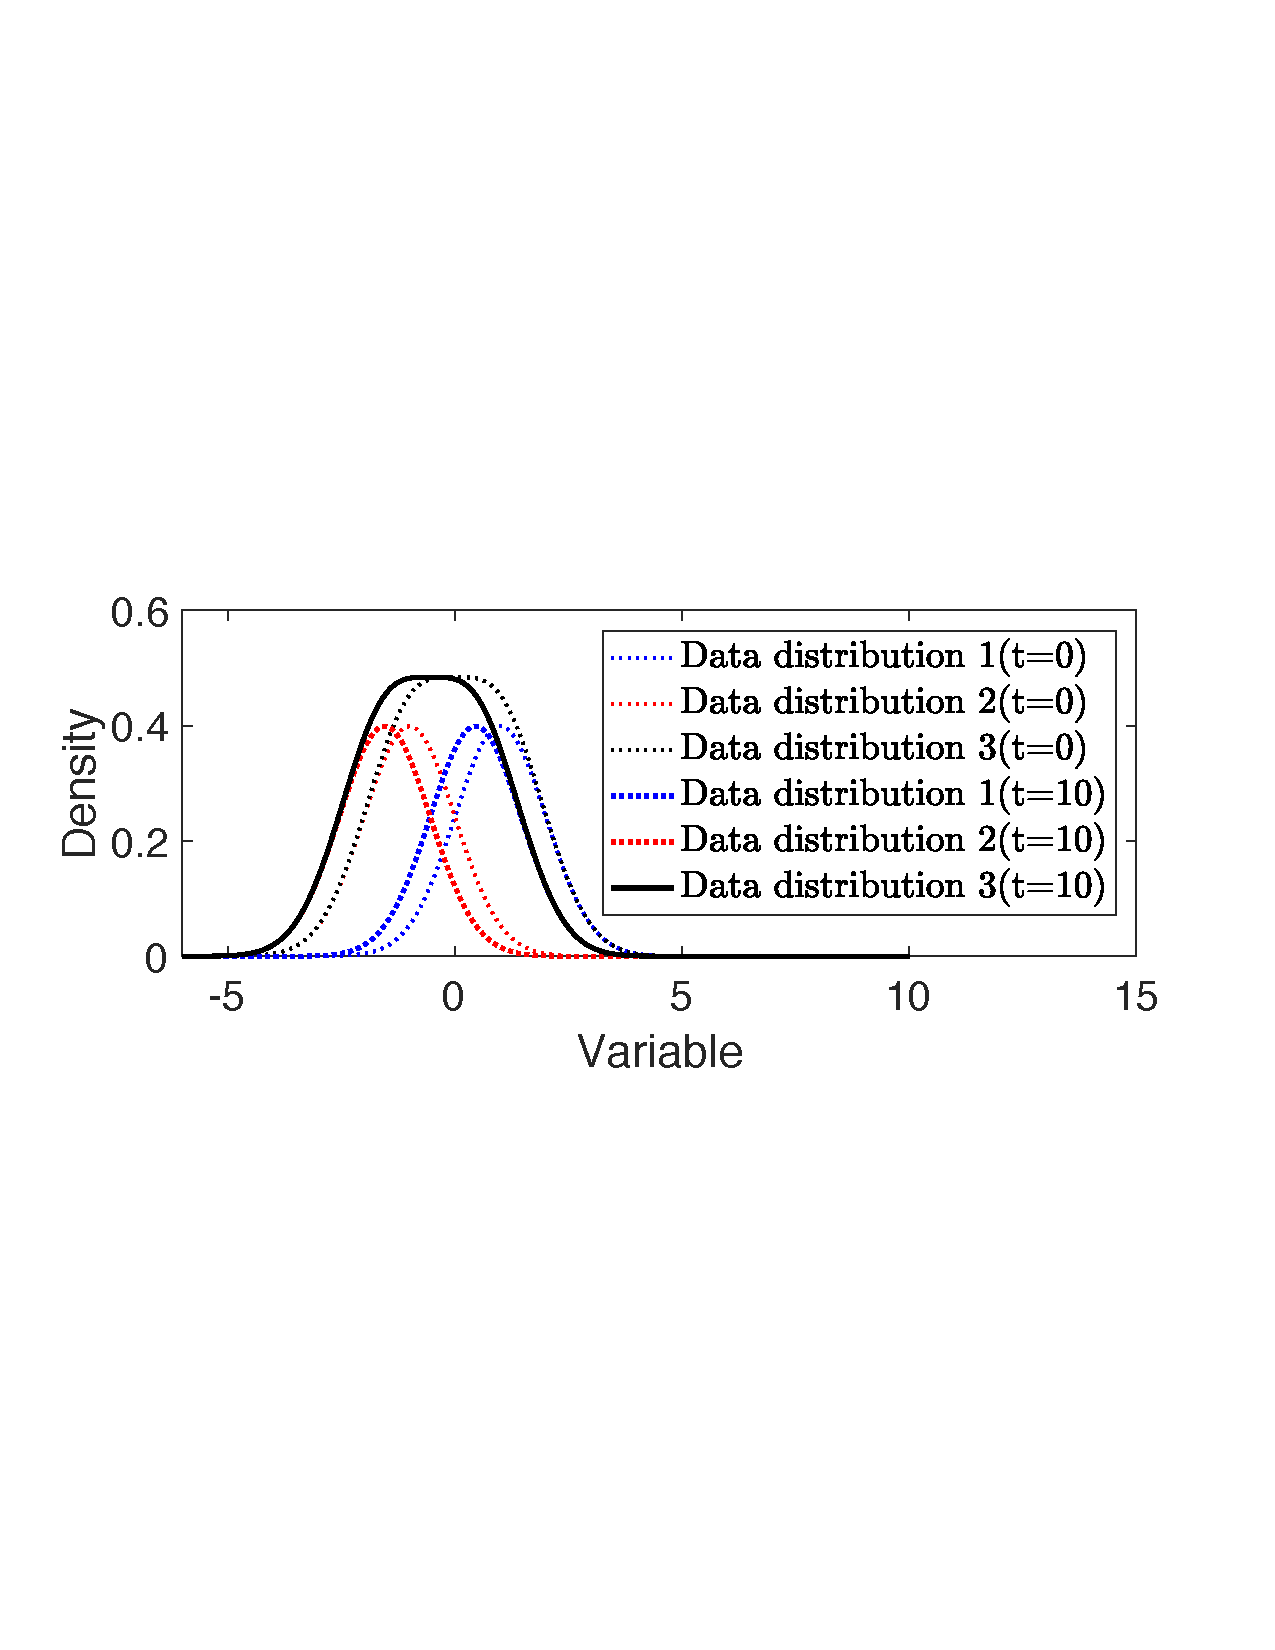
\includegraphics[width=0.9\columnwidth]{figure_dynamics}\label{figure_dynamics}}
\caption{An illustration of the dynmaics caused by the time-varying distributions of data. Data distributions $1$ and $2$ satisify $N(1+\sin(t), 1)$ and $N(-1+\sin(t), 1)$, respectively.  Suppose we want to conduct classification between data drawn from distributions $1$ and $2$, respectively. The optimal classification model should change over time.}
\label{figure_illus_dynamics}
\end{figure}


\begin{figure*}[!h]
\setlength{\abovecaptionskip}{0pt}
\setlength{\belowcaptionskip}{0pt}
\centering 
\subfigure[\textit{synthetic data}, $10000$ nodes,stochastic topology]{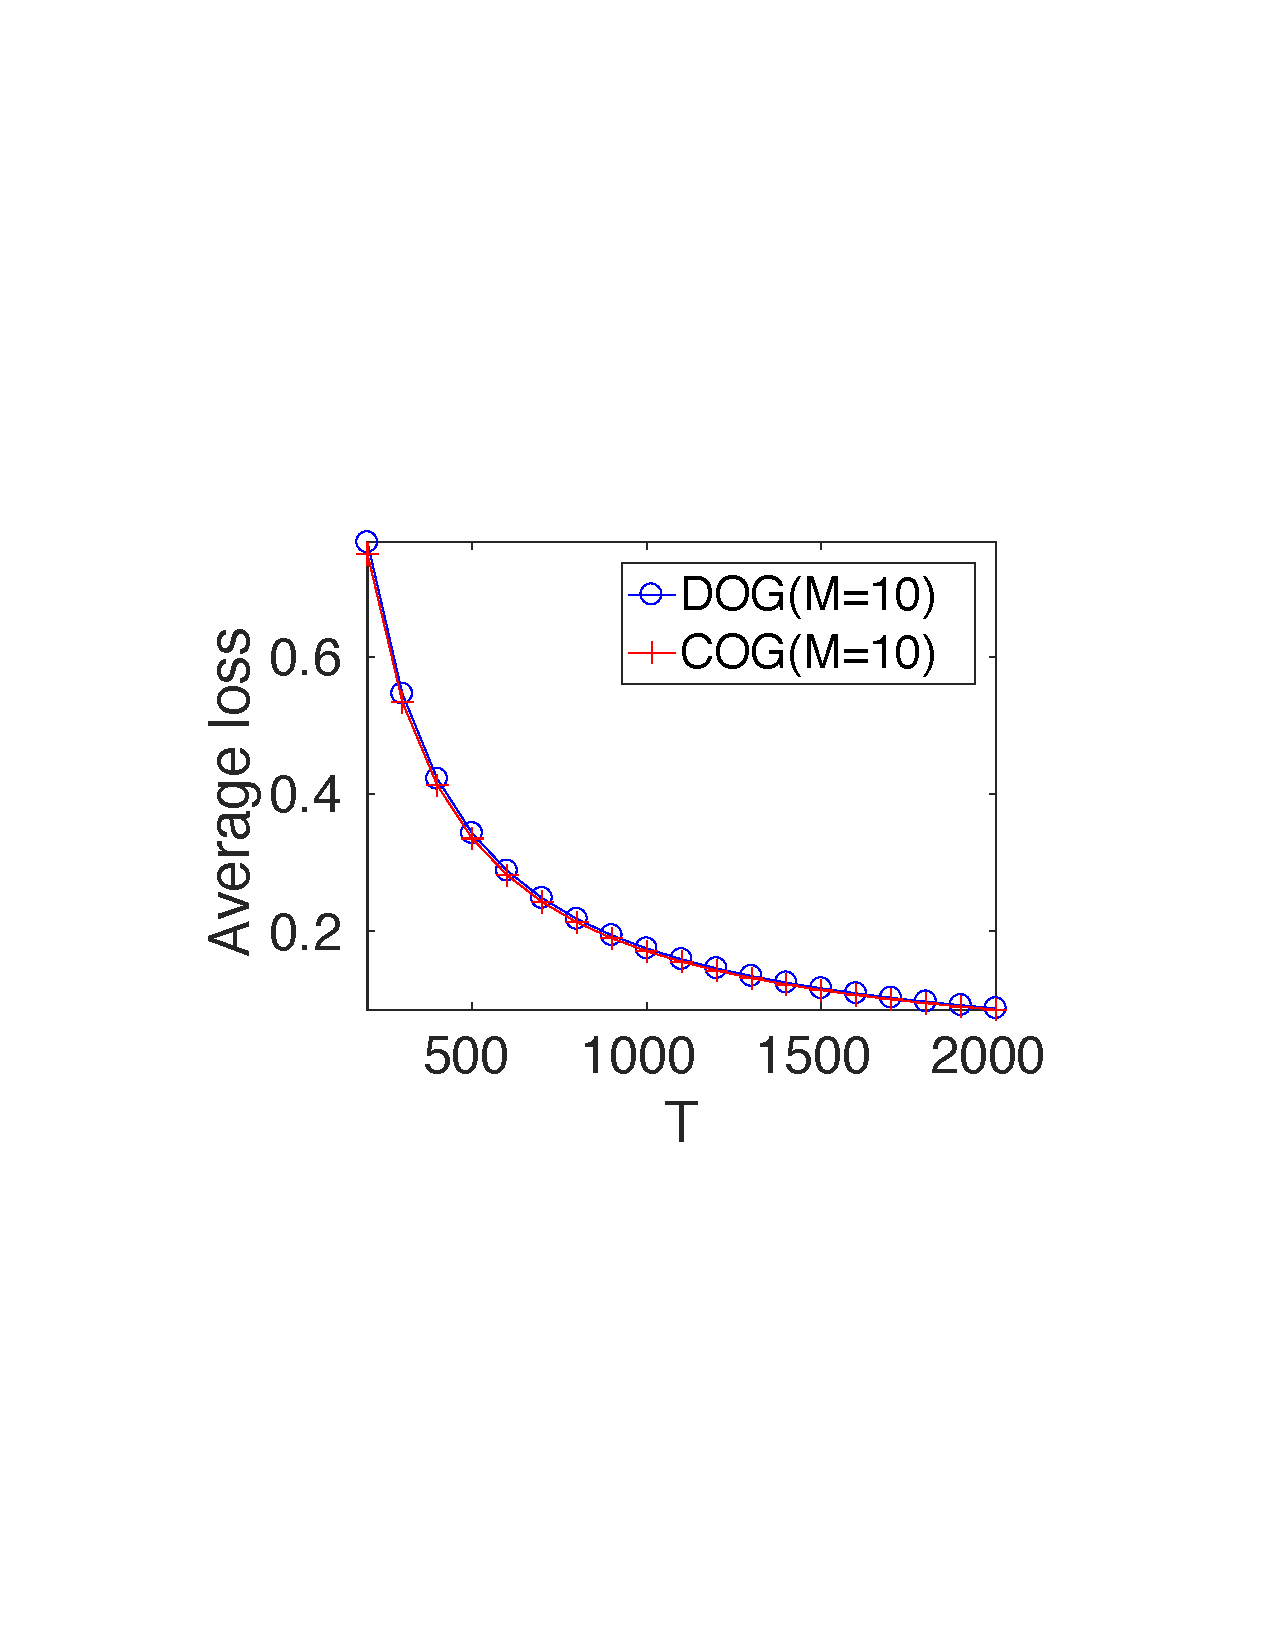
\includegraphics[width=0.48\columnwidth]{figure_ave_loss_iteration_synthetic}\label{figure_ave_loss_iteration}}
\subfigure[\textit{room-occupancy}, $5$ nodes, ring topology]{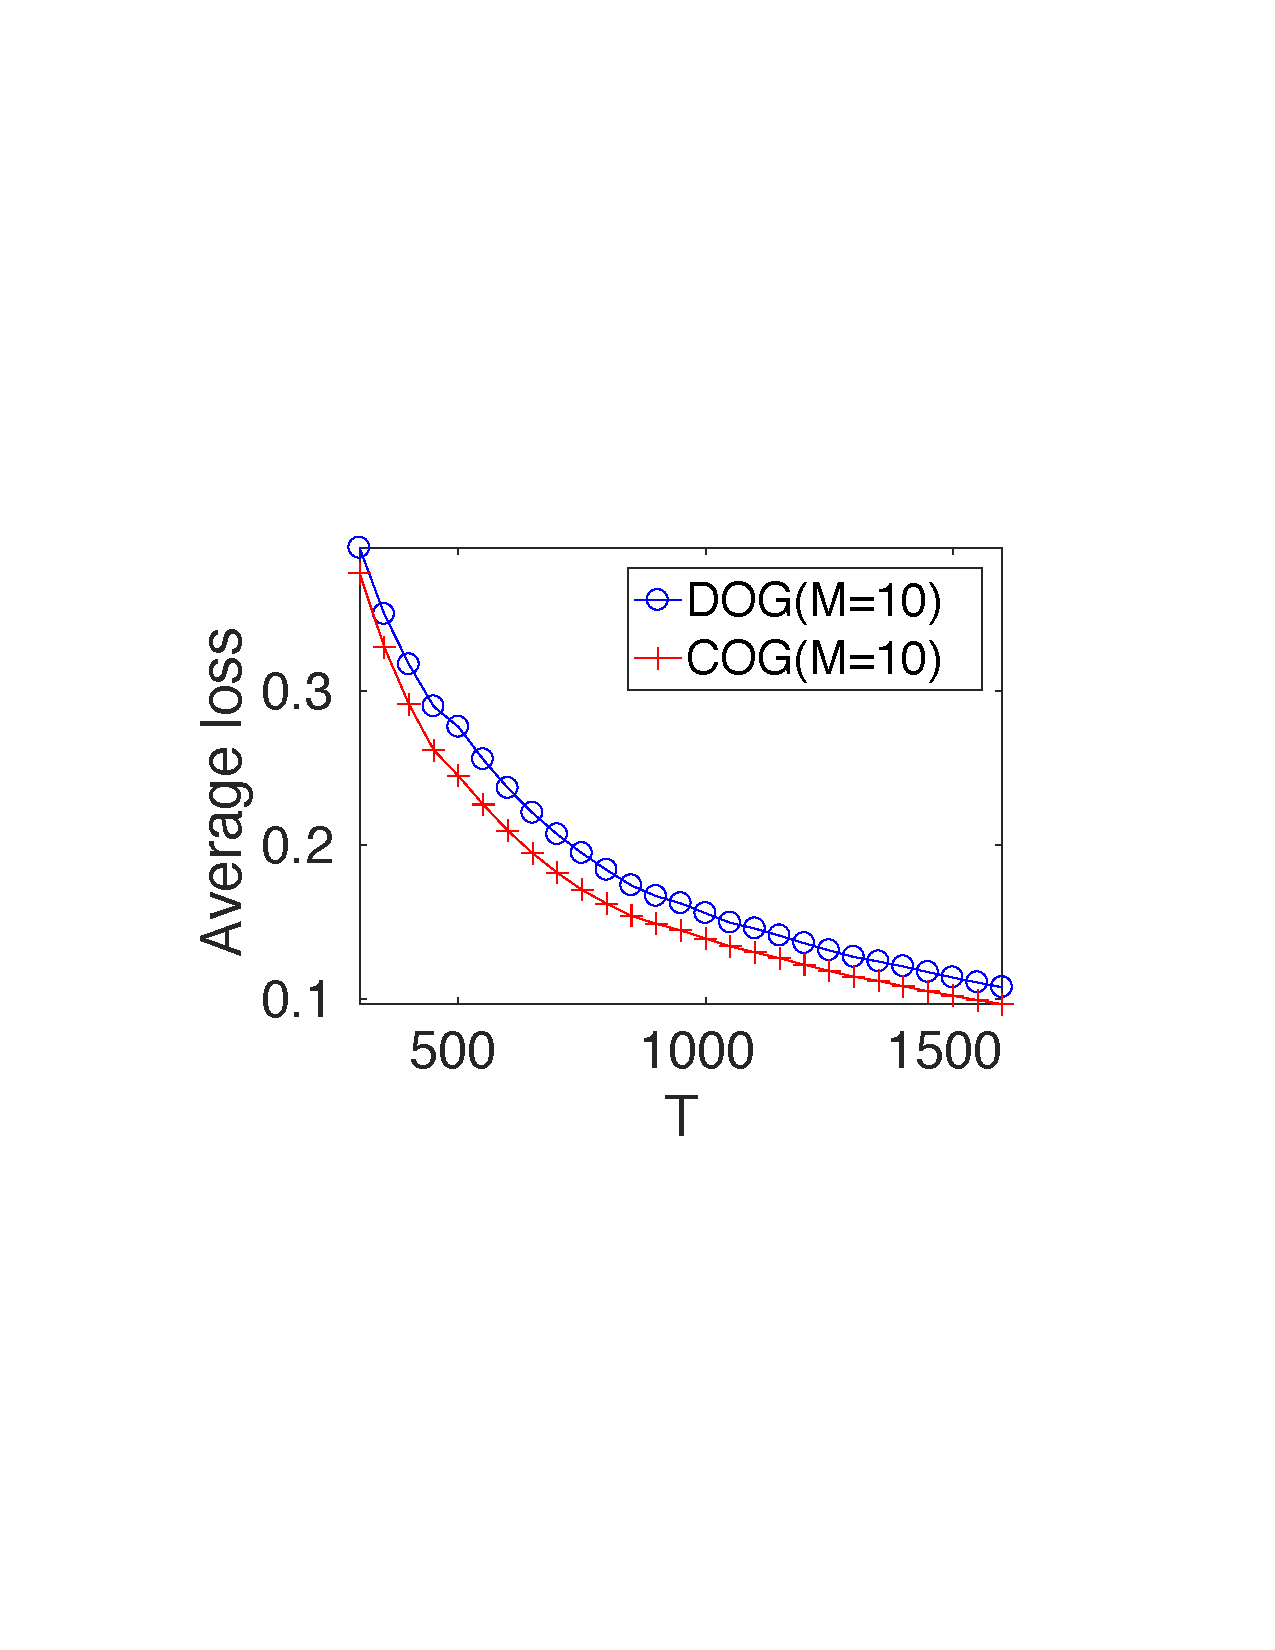
\includegraphics[width=0.48\columnwidth]{figure_ave_loss_iteration_occupancy}\label{figure_ave_loss_iteration_occupancy}}
\subfigure[\textit{usenet2}, $5$ nodes, ring topology]{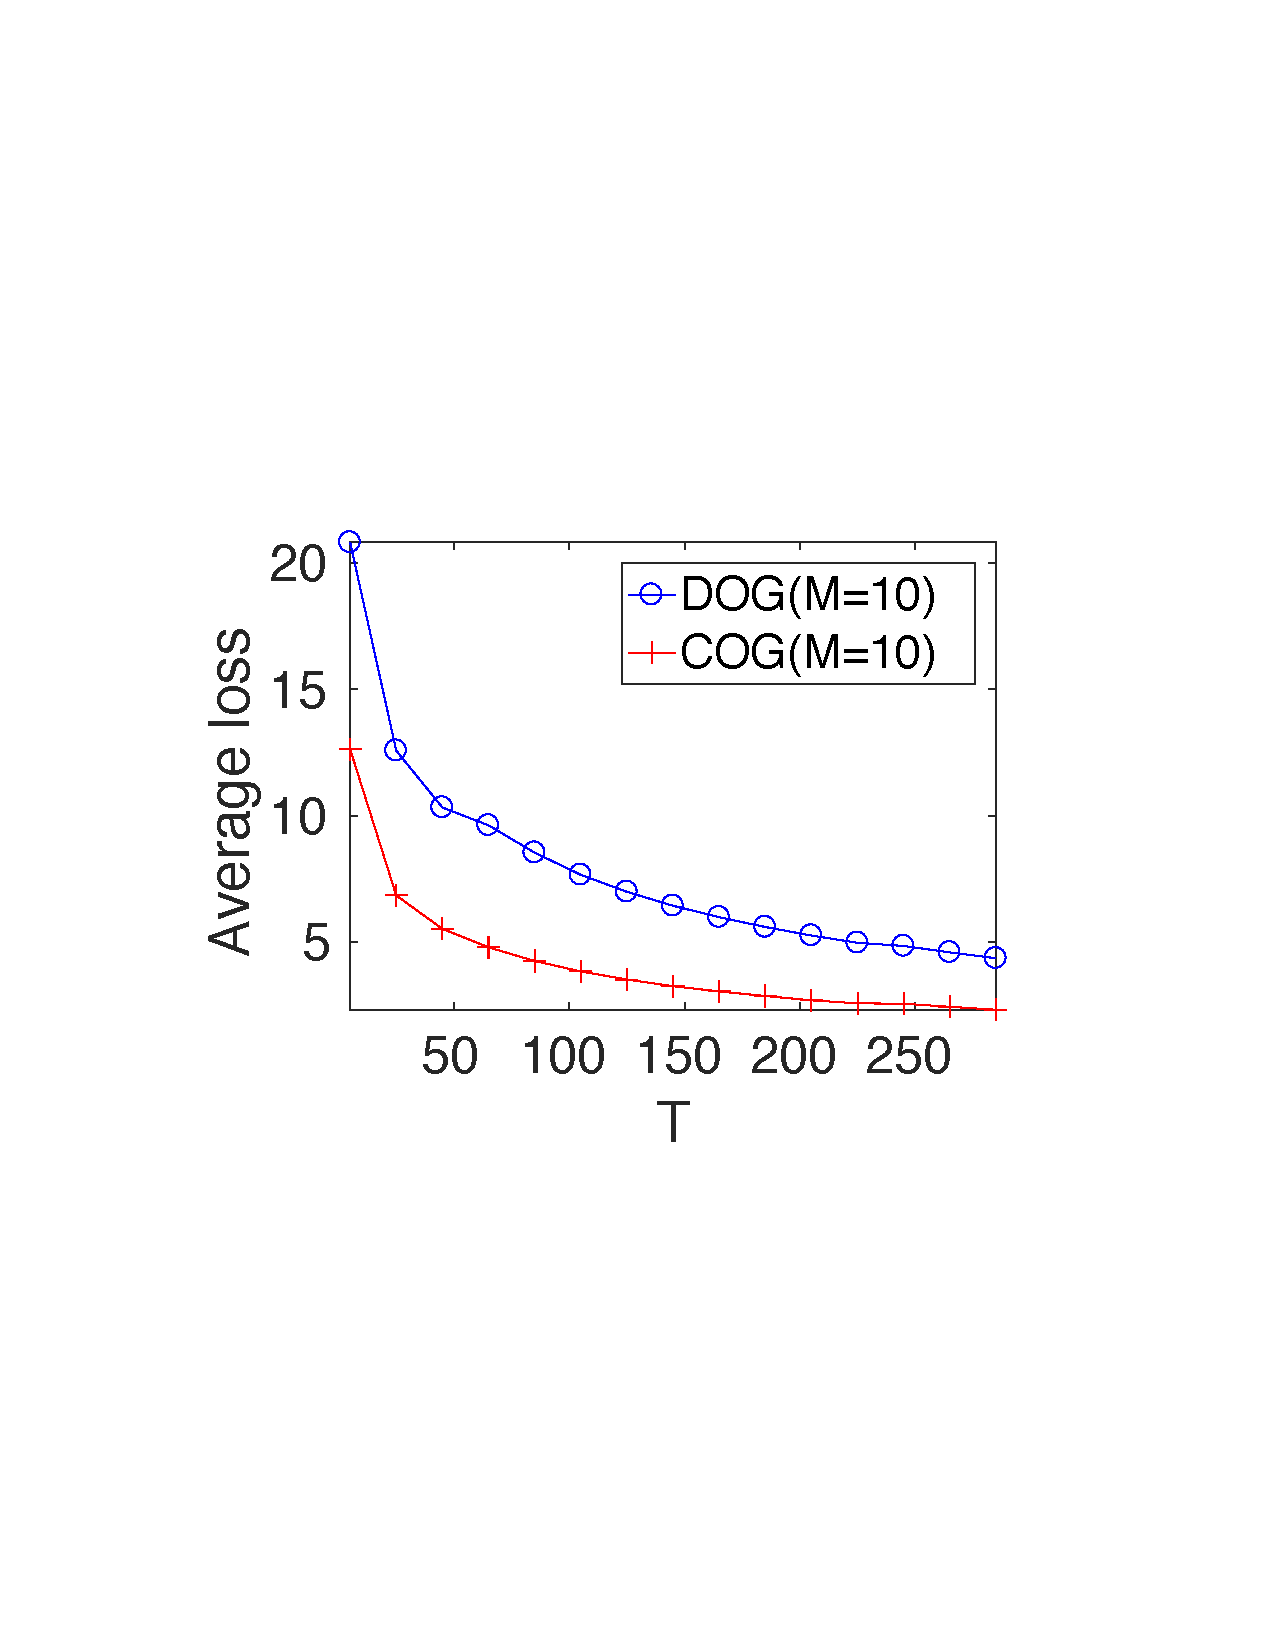
\includegraphics[width=0.48\columnwidth]{figure_ave_loss_iteration_usenet2}\label{figure_ave_loss_iteration_usenet2}}
\subfigure[\textit{spam}, $5$ nodes, ring topology]{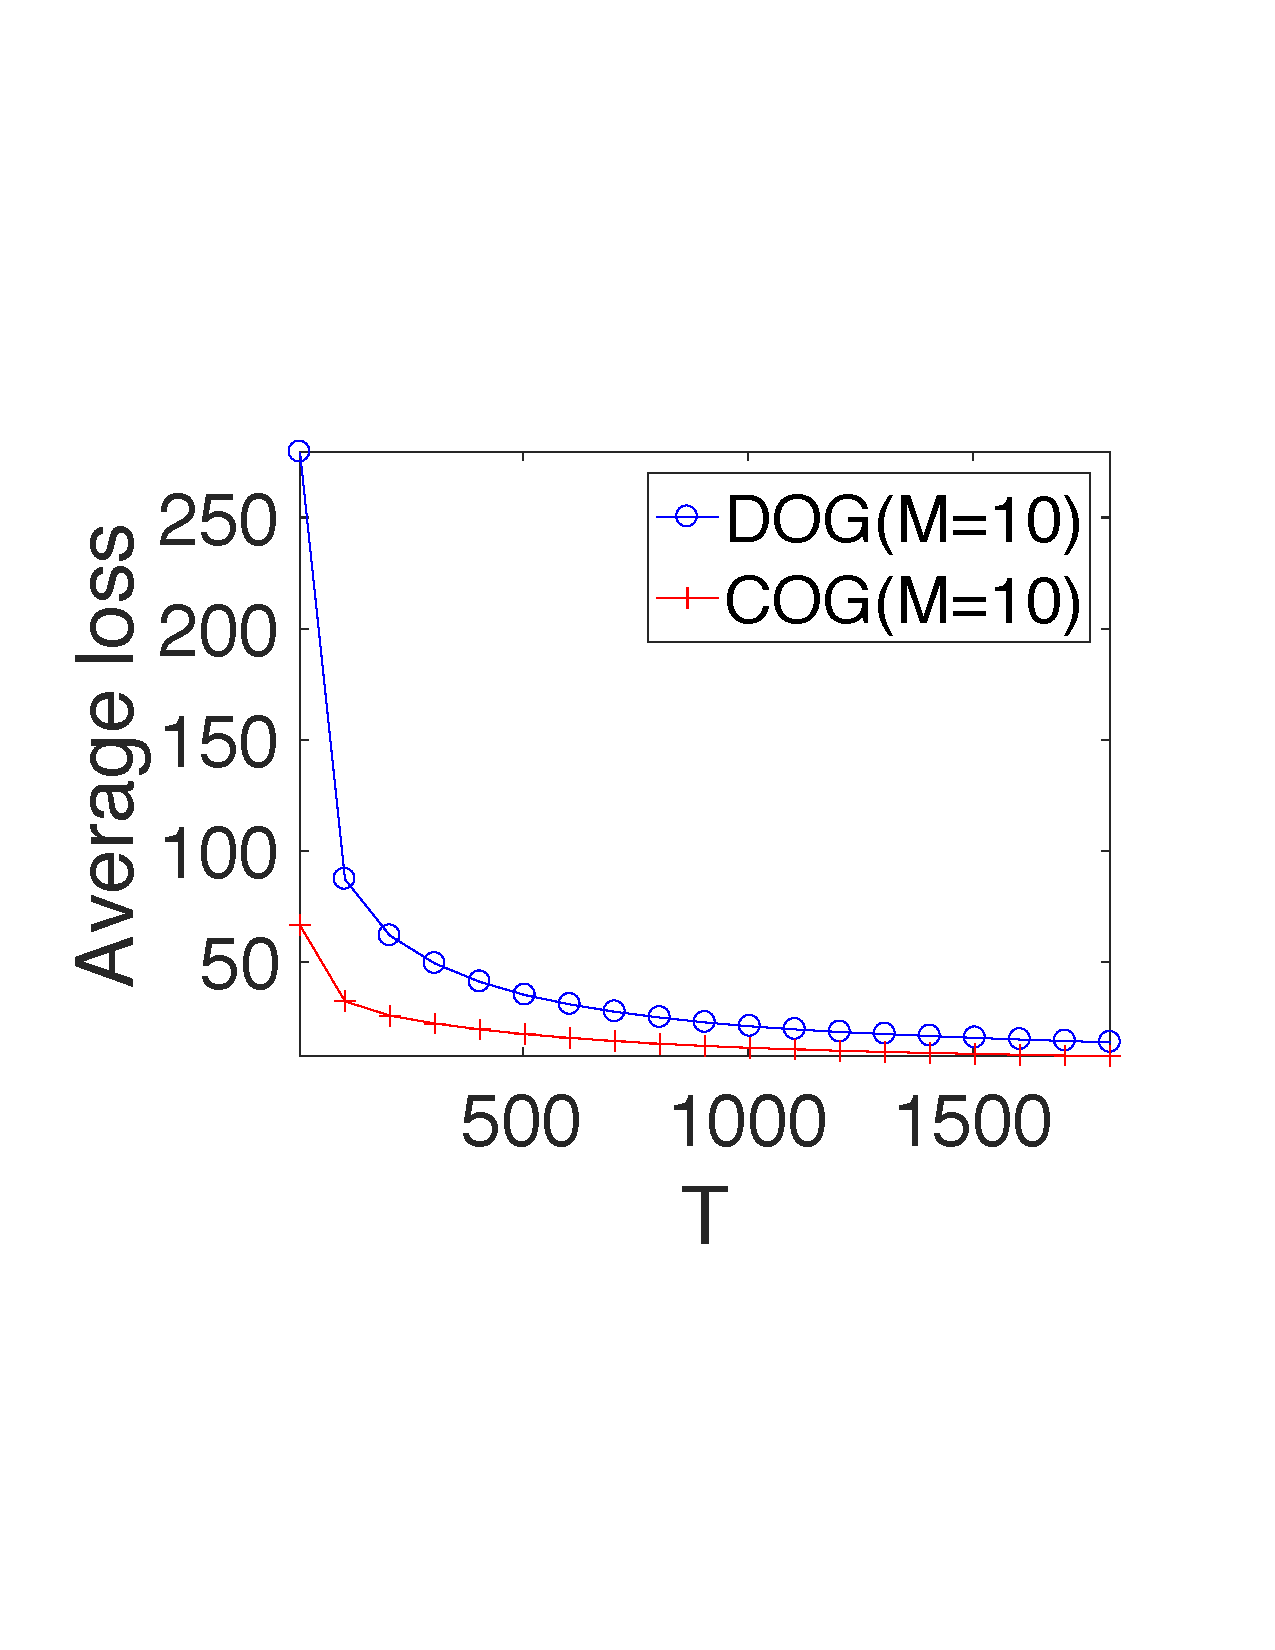
\includegraphics[width=0.48\columnwidth]{figure_ave_loss_iteration_spam}\label{figure_ave_loss_iteration_spam}}
%\subfigure[\textit{usenet2}]{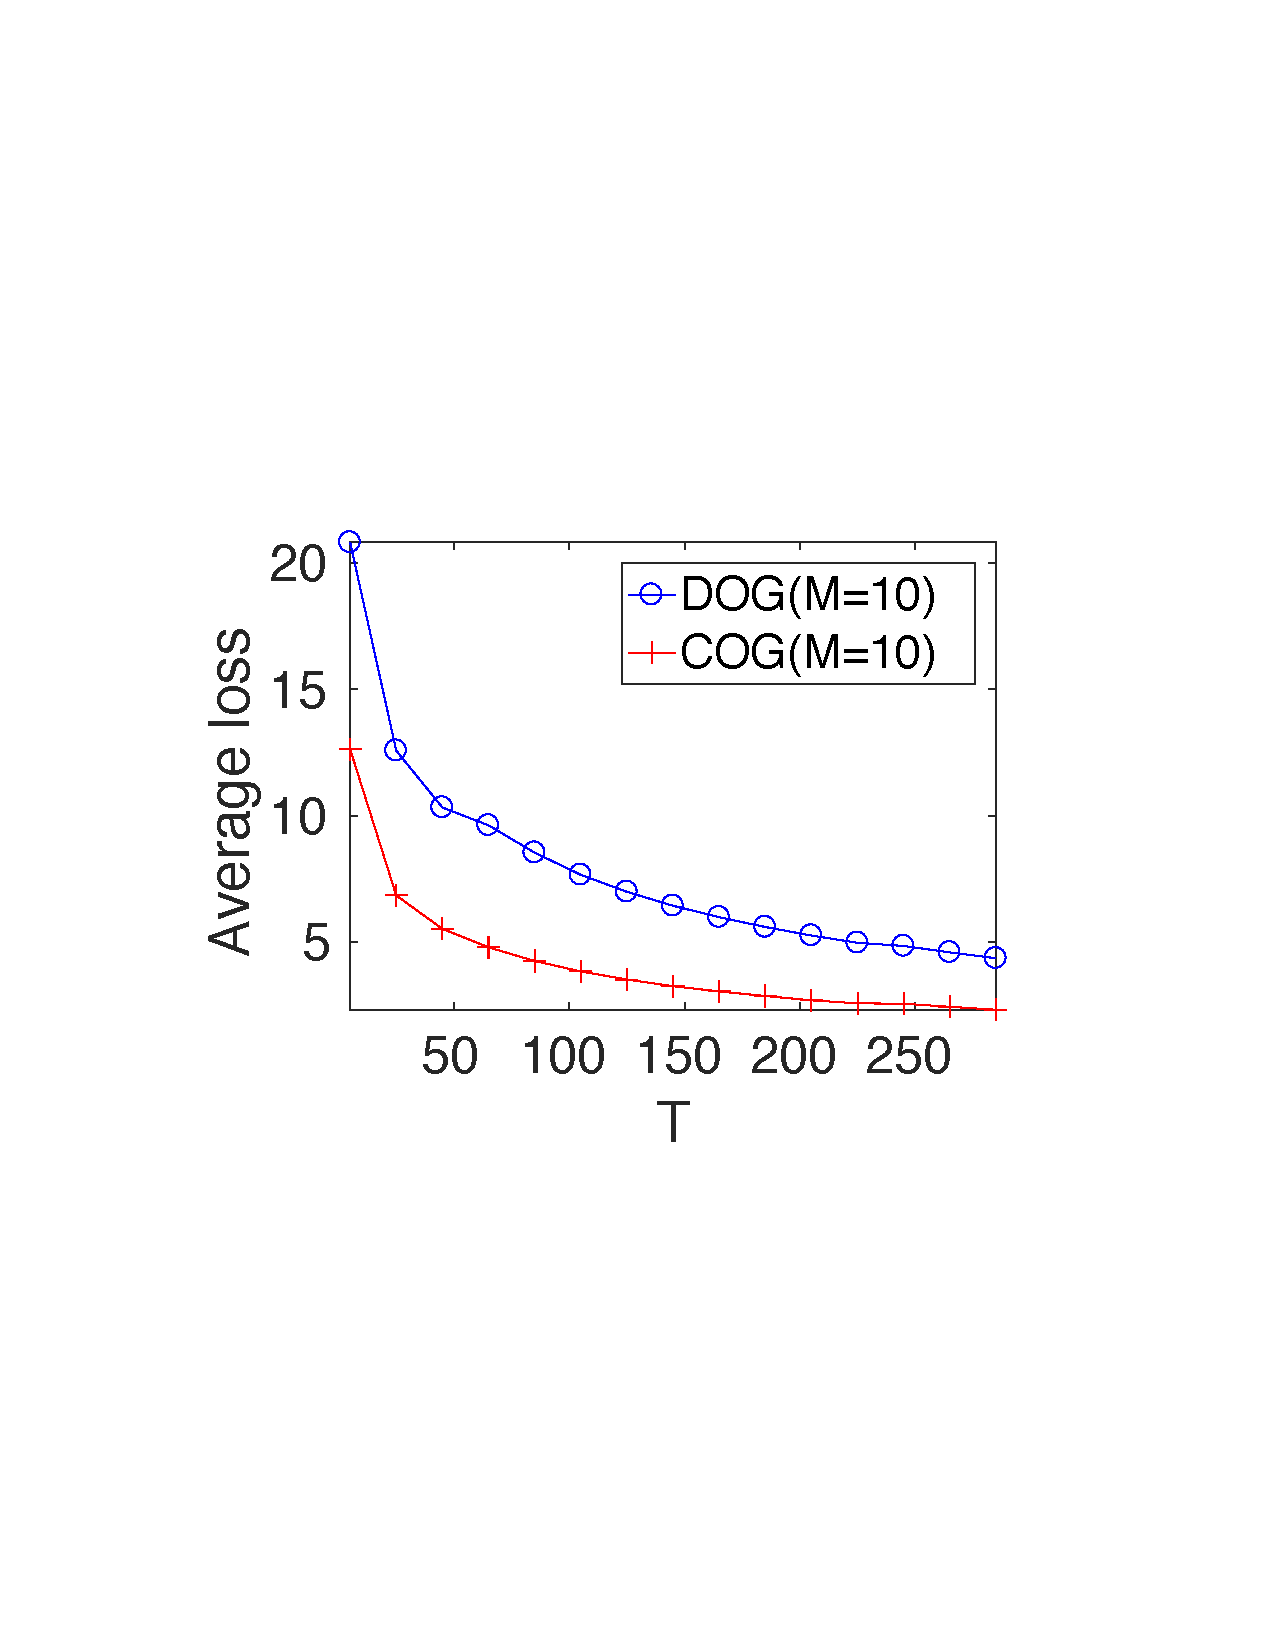
\includegraphics[width=0.32\columnwidth]{figure_ave_loss_iteration_usenet2}\label{figure_ave_loss_iteration_usenet2}}
\caption{The average loss yielded by DOG is comparable to that yielded by COG.}
\label{figure_compare_loss}
\end{figure*}




To test the proposed algorithm, we utilized a toy dataset and three real-world datasets, whose details are presented as follows.

\textbf{Synthetic Data} 
For the $i$-th node, a data matrix  $\A_i\in R^{10\times T}$ is generated, s.t. $\A_i=0.1\tilde{\A}_i+0.9\hat{\A}_i$, where $\tilde{\A}_i$ represents the adversary part of data, and $\hat{\A}_i$ represents the stochastic part of data. Specifically,  elements of $\tilde{\A}_i$ is uniformly sampled from the interval $[-0.5+\sin(i),0.5+\sin(i)]$. Note that $\tilde{\A}_i$ and $\tilde{\A}_j$ with $i\neq j$ are drawn from different distributions. $\hat{\A}_{i,t}$ is generated according to $\y_{i,t}\in\{1,-1\}$ which is generated uniformly. When $\y_{i,t}=1$, $\hat{\A}_{i,t}$ is generated by sampling from a time-varying distribution $N((1+0.5\sin(t))\cdot\1, \I)$. When $\y_{i,t} = -1$, $\hat{\A}_{i,t}$ is generated by sampling from another time-varying distribution $N((-1+0.5\sin(t))\cdot\1, \I)$. Due to this correlation, $y_{i,t}$ can be considered as the label of the instance $\hat{\A}_{i,t}$.
The above dynamics of time-varying distributions are illustrated in Figure~\ref{figure_illus_dynamics}, which shows the change of the optimal learning model over time and the importance of studying the dynamic regret. 

\textbf{Real Data}
Three real public datasets are \textit{room-occupancy}\footnote{\url{https://archive.ics.uci.edu/ml/datasets/Occupancy+Detection+}},  \textit{usenet2}\footnote{\url{http://mlkd.csd.auth.gr/concept_drift.html}}, and \textit{spam}\footnote{\url{http://mlkd.csd.auth.gr/concept_drift.html}}. \textit{room-occupancy} is a time-series dataset, which is from a natural dynamic enviroment. Both \textit{usenet2} and \textit{spam} are  ``concept drift" \citep{Katakis:2010:TR} datasets, for which the optimal model changes over time.   

%Besides, we fetch values of the first feature of every dataset, and then permutate them by the decreasing order. After that, we re-fill the new values to the data matrix to simulate the adversary values. Finally, all values of a feature have been normalized to be zero mean and one variance.
%\begin{itemize}
%\item {\textit{room-occupancy}.} It collects features of a room including temperature, humidity, light, and CO2 for every minute between 02/02/2015 and 02/10/2015. Label of an instance is whether the room is occupied. Our goal is to learn a classification model to make a decision whether the room is occupied by using those features.   
%\item {\textit{usenet2}.} It is an online retail dataset, which contains all transactions occurring between 01/12/2010 and 09/12/2011 for a UK-based and registered non-store online retail. We use three features, that is, \textit{whether a transaction is cancelled}, \textit{quantity}, and \textit{unit price}. We need to train a binary clssification model to make a decision whether a customer is coming from United Kingdom. 
%\item {\textit{BeijingPM2.5}.} It collects some weather features, e.g., teperature and pressure, and the PM2.5 data of US Embassy in Beijing hourly between 01/01/2010 and 12/31/2014. When the PM 2.5 index is larger than $100$, the air quality is \textit{bad}, otherwise, \textit{good}. We want to train a binary clssification model to make a decision whether the air quality is good accoring to features such as temperature and pressure.   \textit{BeijingPM2.5}\footnote{\url{https://archive.ics.uci.edu/ml/datasets/Beijing+PM2.5+Data}},
%\item {\textit{spam}.} Every instance in the dataset is an email, where the frequence of every word in the dictionary is collected. But, the distribution of words changes over time, which is denoted by \textit{concept drift} \citep{Katakis:2010:TR}. We want to learn a classification model to make a decision whether an email is a spam. 
%\end{itemize}


\subsection{Results}

First, DOG yields comparable performance with COG. Figure~\ref{figure_compare_loss} summarizes the performance of DOG compared with COG on all the datasets. 
For the synthetic dataset, we simulated a decentralized network consisting of $10000$ nodes, where every node is stochasticly connected with other $15$ nodes.
For the three real datasets, we simulated a network consisting of $5$ nodes. 
In these networks, the nodes are connected by a ring topology. 
Under these settings, we can observe that both DOG and COG are effective for the online learning tasks on all the datasets, while DOG achieves slightly worse performance. 


Second, the performance of DOG is not sensitive to the network size, but sensitive to the variance of the stochastic data. Figure~\ref{figure_compare_network_size} summarizes the effect of the network size on the performance of DOG. We change the number of nodes from $5000$ to $10000$ on the synthetic dataset, and from $5$ to $20$ on the real datasets. The synthetic dataset is tested by using the stochastic topology, and those real datasets are tested by using the ring topology. Figure~\ref{figure_compare_network_size} draws the curves of average loss over time steps. We observe that the average loss curves are mostly overlapped with different nodes. It shows that DOG is robust to the network size (or number of users), which validates our theory, that is, the average regret does not increase with the number of nodes. Furthermore, we observe that the average loss becomes large with the increase of the variance of stochastic data, which validates our theoretical result nicely.  


\begin{figure*}[!h]
\setlength{\abovecaptionskip}{0pt}
\setlength{\belowcaptionskip}{0pt}
\centering 
\subfigure[\textit{synthetic data}, stochastic topology]{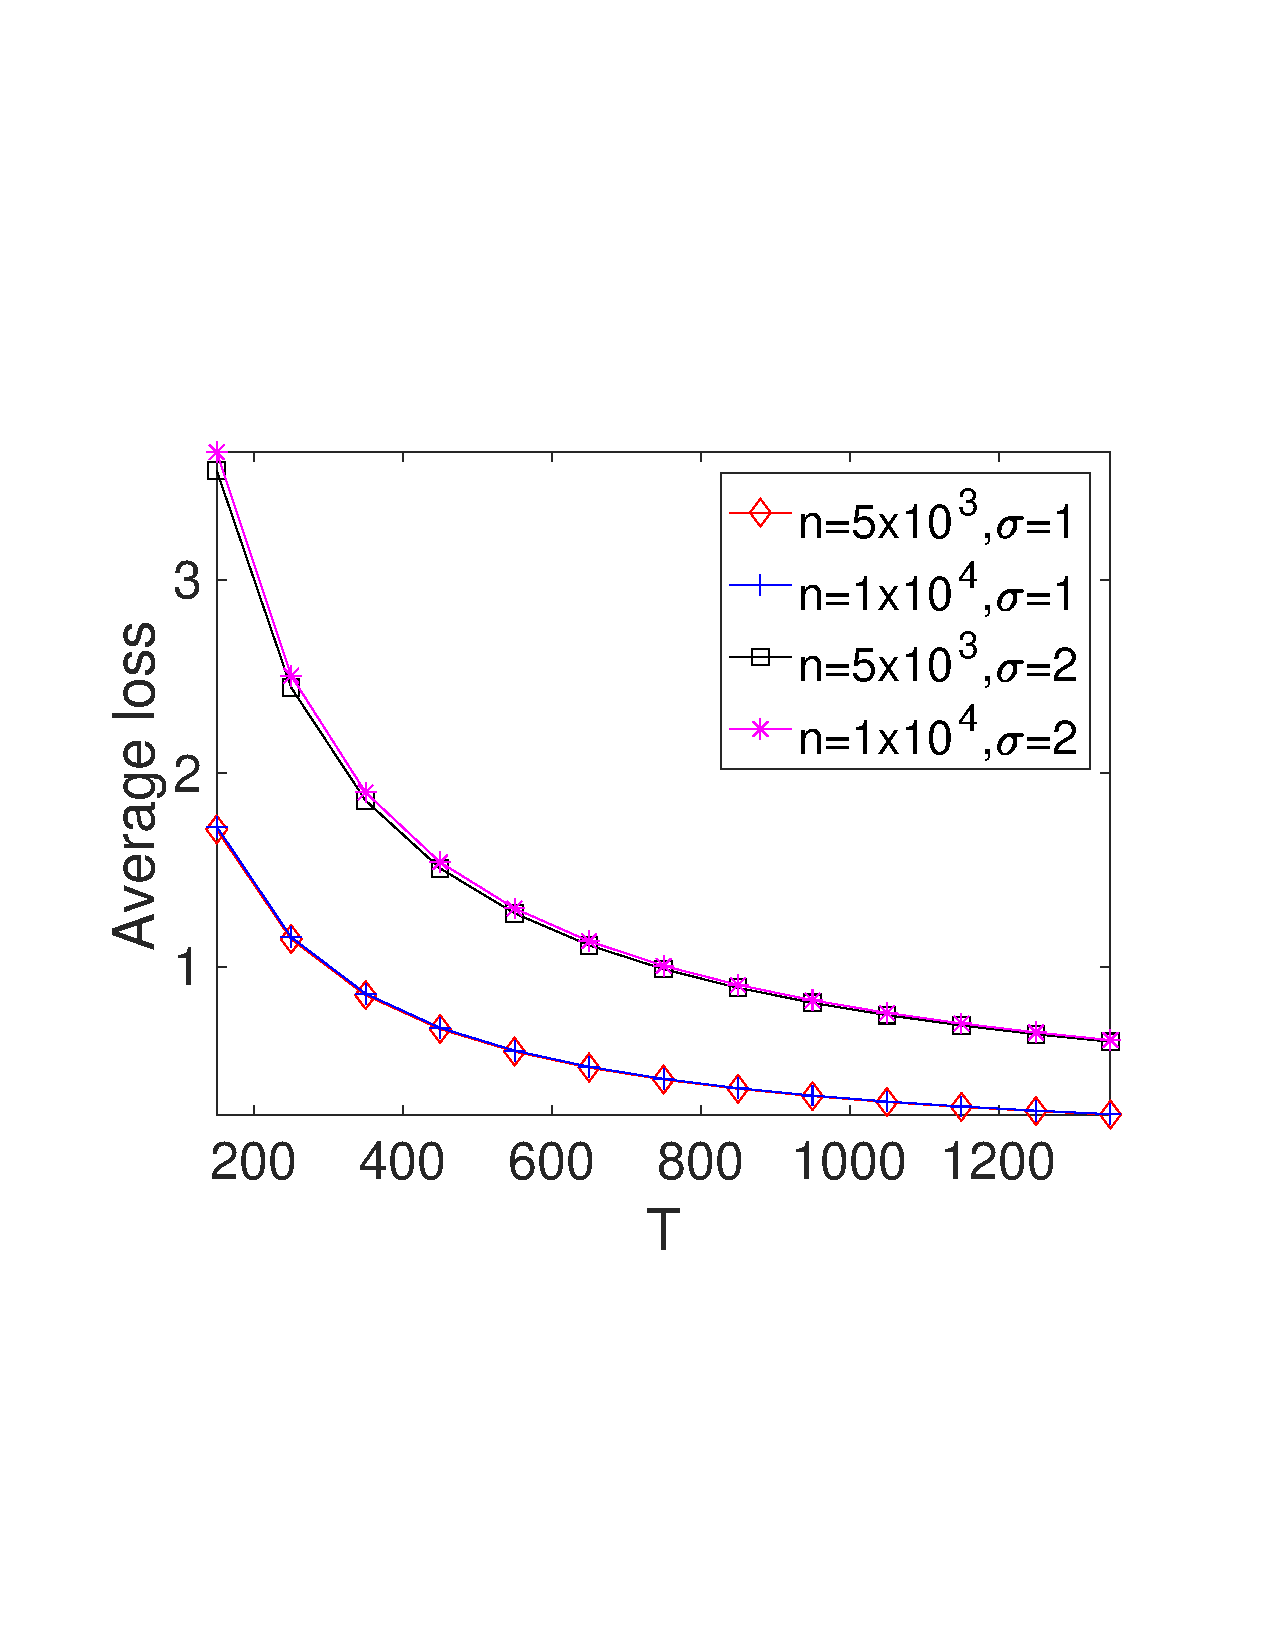
\includegraphics[width=0.48\columnwidth]{figure_ave_loss_network_size_synthetic}\label{figure_ave_loss_network_size_synthetic}}
\subfigure[\textit{room-occupancy}, ring topology]{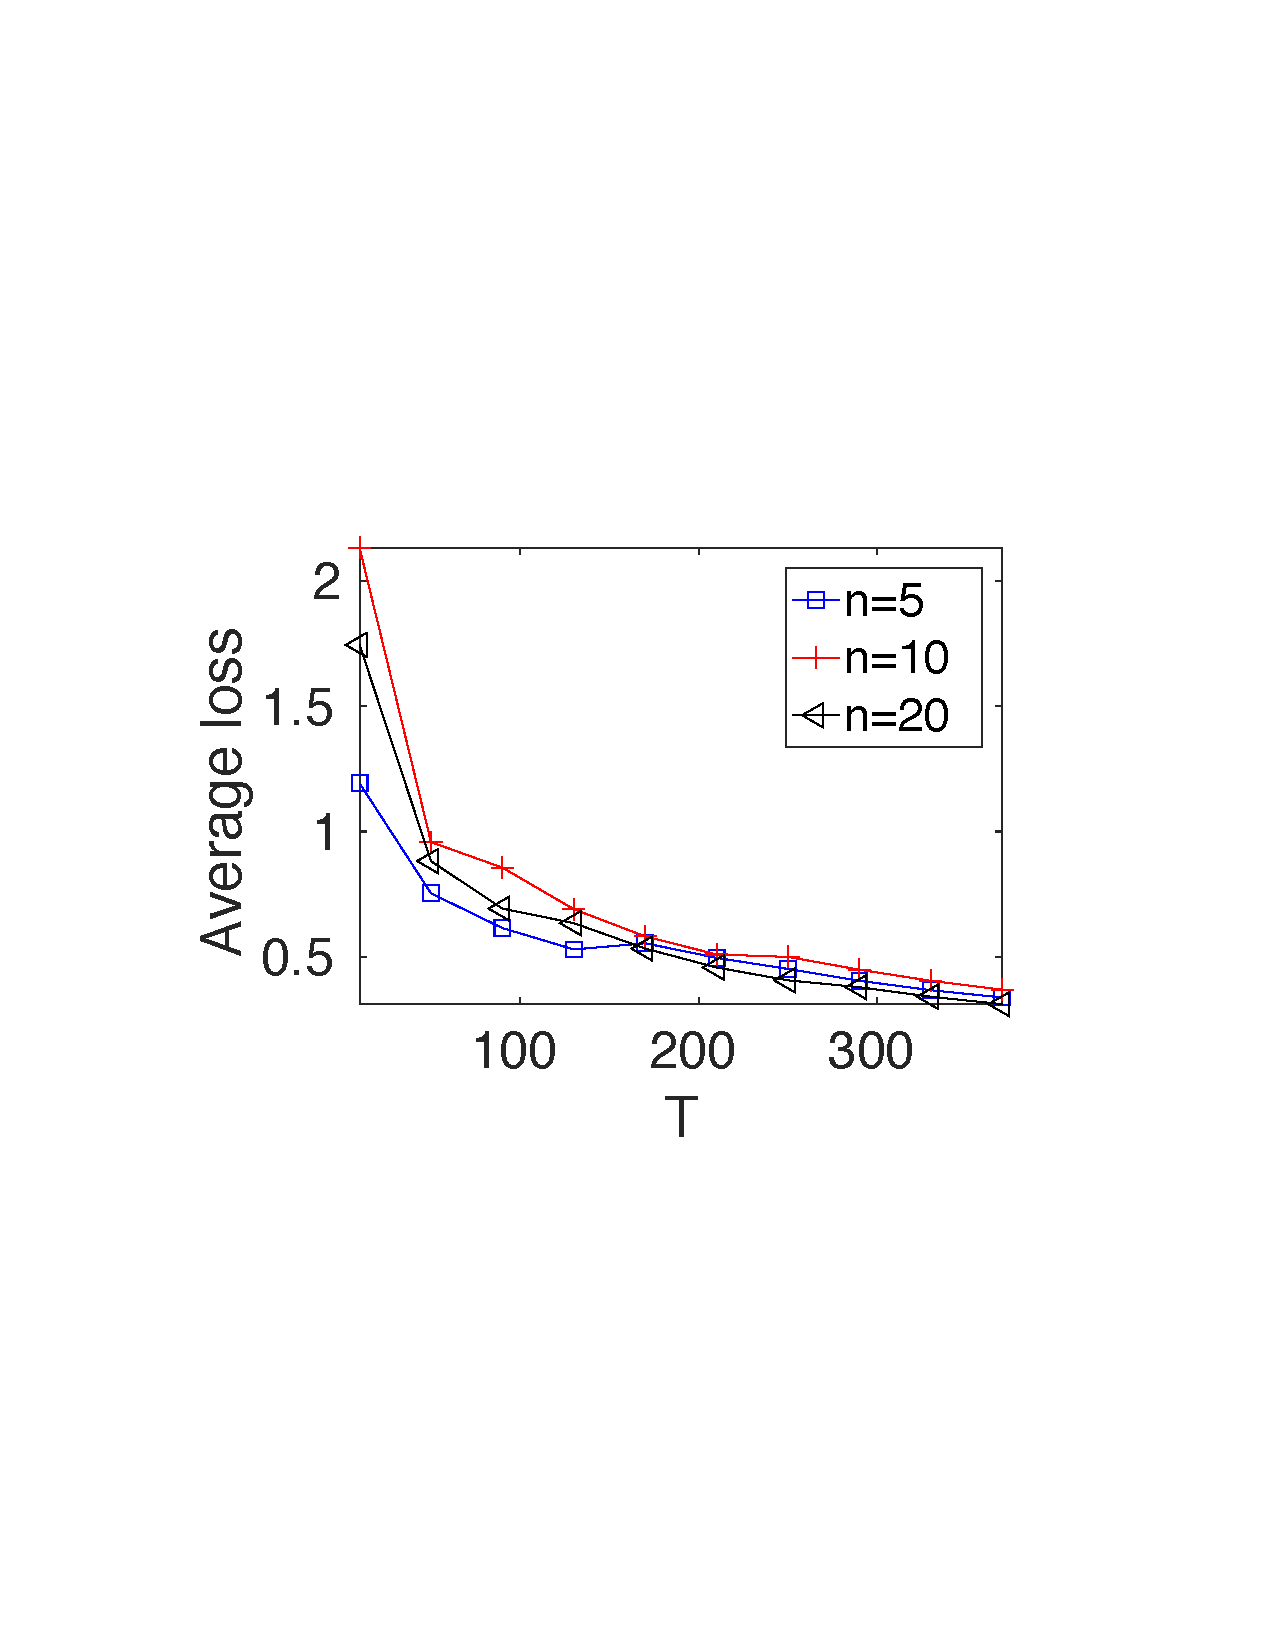
\includegraphics[width=0.48\columnwidth]{figure_ave_loss_network_size_occupancy}\label{figure_ave_loss_network_size_occupancy}}
\subfigure[\textit{usenet2}, ring topology]{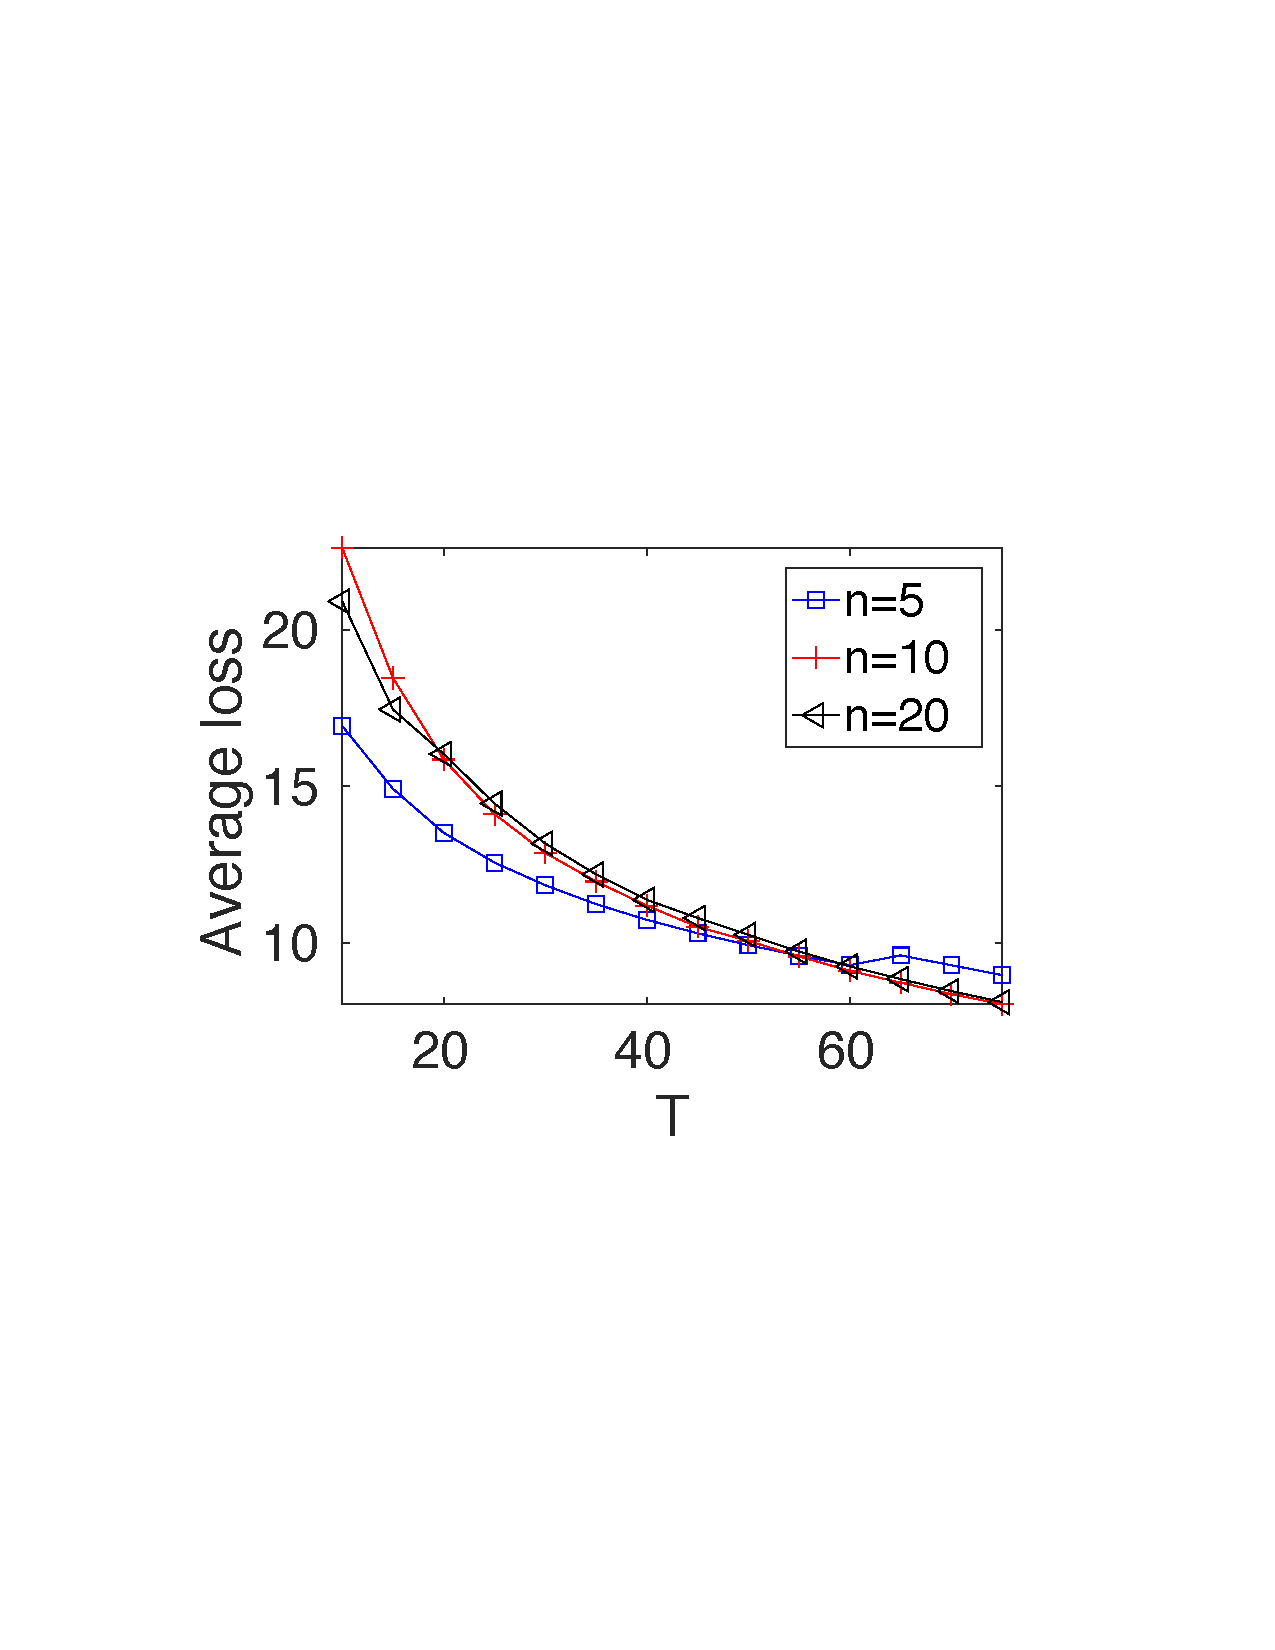
\includegraphics[width=0.48\columnwidth]{figure_ave_loss_network_size_usenet2}\label{figure_ave_loss_network_size_usenet2}}
\subfigure[\textit{spam}, ring topology]{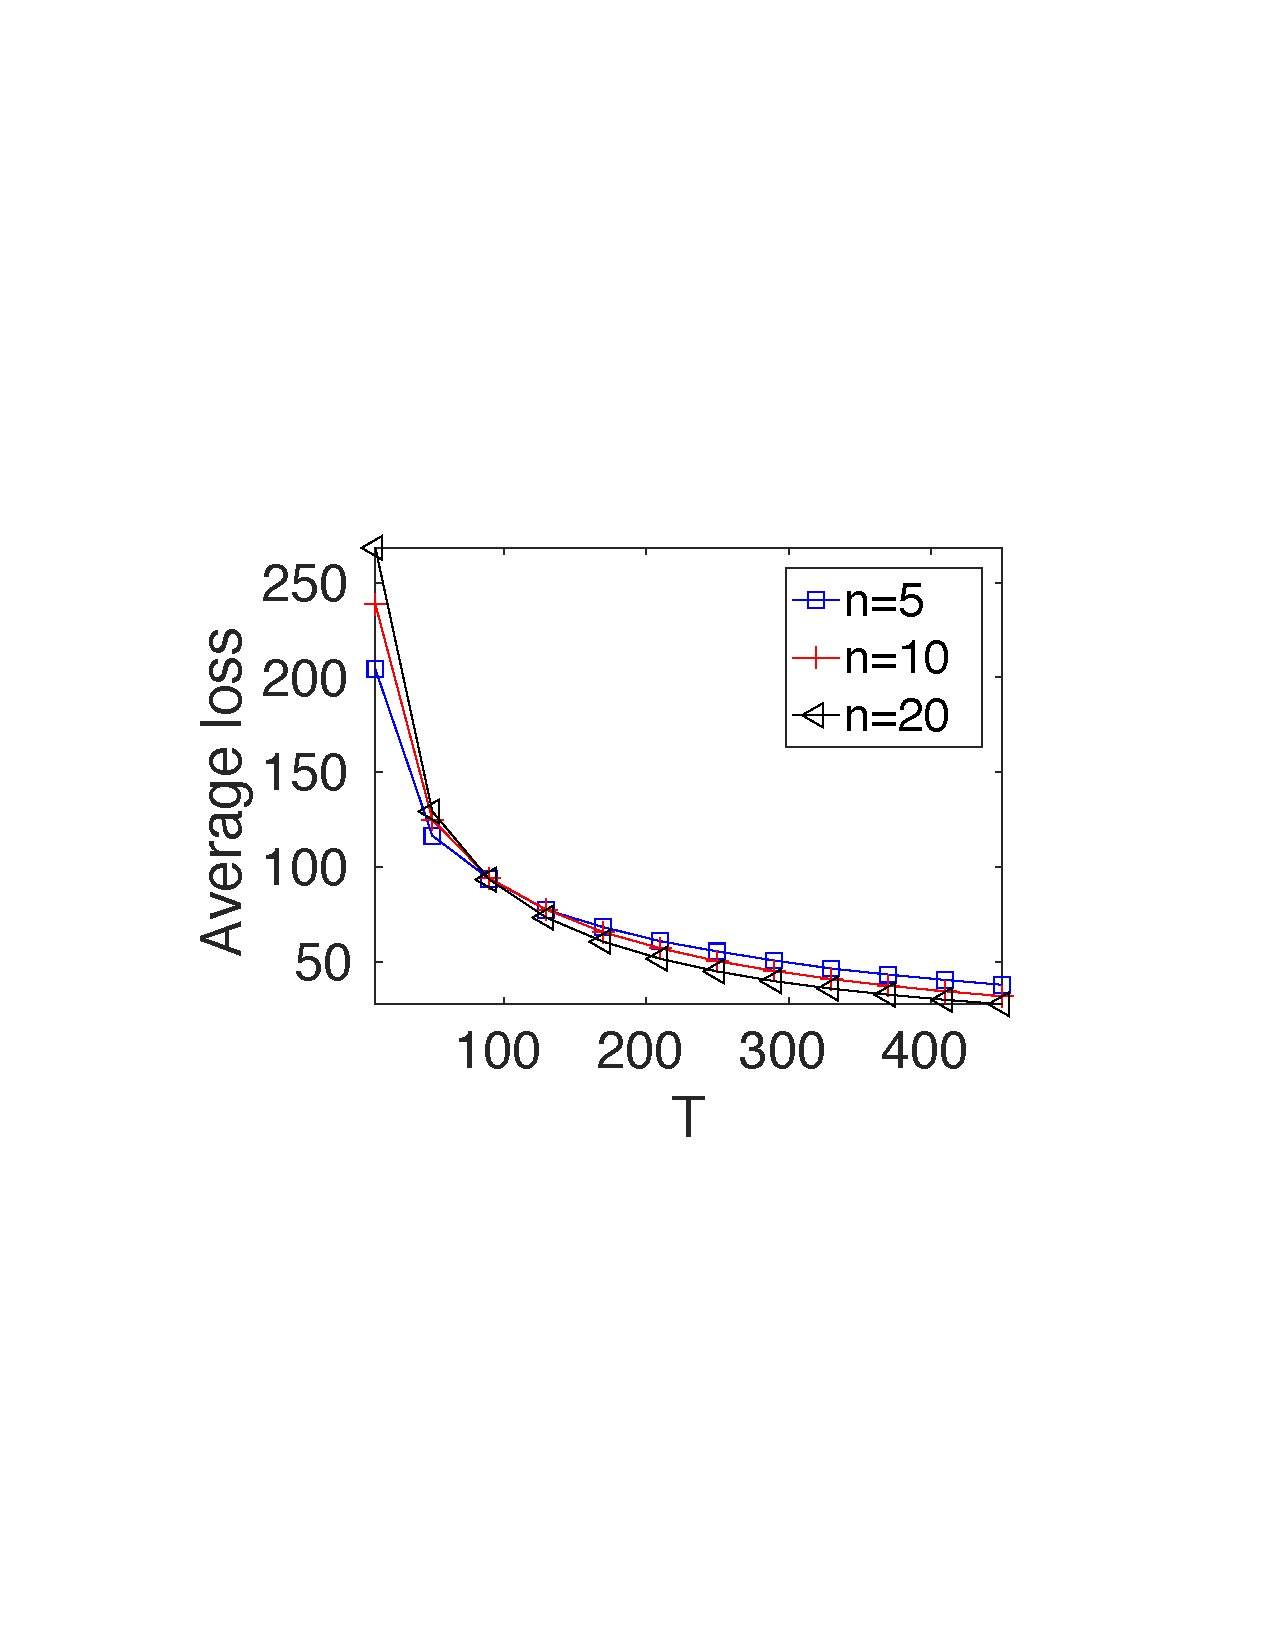
\includegraphics[width=0.48\columnwidth]{figure_ave_loss_network_size_spam}\label{figure_ave_loss_network_size_spam}}
\caption{The average loss yielded by DOG is insensitive to the network size.}
\label{figure_compare_network_size}
\end{figure*}


Third, the performance DOG is improved in a well-connected network. Figure~\ref{figure_compare_topology} shows the effect of the topology of the network on the performance of DOG, where five different topologies are used. Besides the ring topology, the \textit{No connected} topology means there are no edges in the network, and every node does not share its local model to others. The \textit{Fully connected} topology means all nodes are connected, where DOG de-generates to be COG. The topology  \textit{WattsStrogatz} represents a Watts-Strogatz small-world graph, for which we can use a parameter to control the number of stochastic edges (set as $0.5$ and $1$ in this paper). The result shows \textit{Fully connected} enjoys the best performance, because that $\rho = 0$ for it while $\rho>0$ for other topologies. Specifically, $\rho$ in those topologies is presented in Table \ref{table_rho}. A small $\rho$ leads to a good performance of DOG, which validates our theoretical result nicely. 


\begin{table}[!]
\begin{tabular}{c|c|c|c|c|c}
\hline
$\rho$    & NC & FC & Ring & WS($1$) &  Ws($0.5$) \\ \hline  \hline
synthetic data & 1            & 0               &   0.99   &       0.37            &  0.58 \\ \hline
real data     & 1            & 0               &    0.96   &          0.83         &  0.76 \\ \hline
\end{tabular}
\caption{$\rho$ in different topologies used in our experiment. A large $1-\rho$ represents good connectivity of the communication network. ``NC" represents the \textit{No connected} topology, ``FC" represents the \textit{Fully connected} topology, and ``WS" represents the \textit{WattsStrogatz} topology.}
\label{table_rho}
\end{table}

 



\begin{figure*}[!h]
\setlength{\abovecaptionskip}{0pt}
\setlength{\belowcaptionskip}{0pt}
\centering 
\subfigure[\textit{synthetic data}, $10000$ nodes]{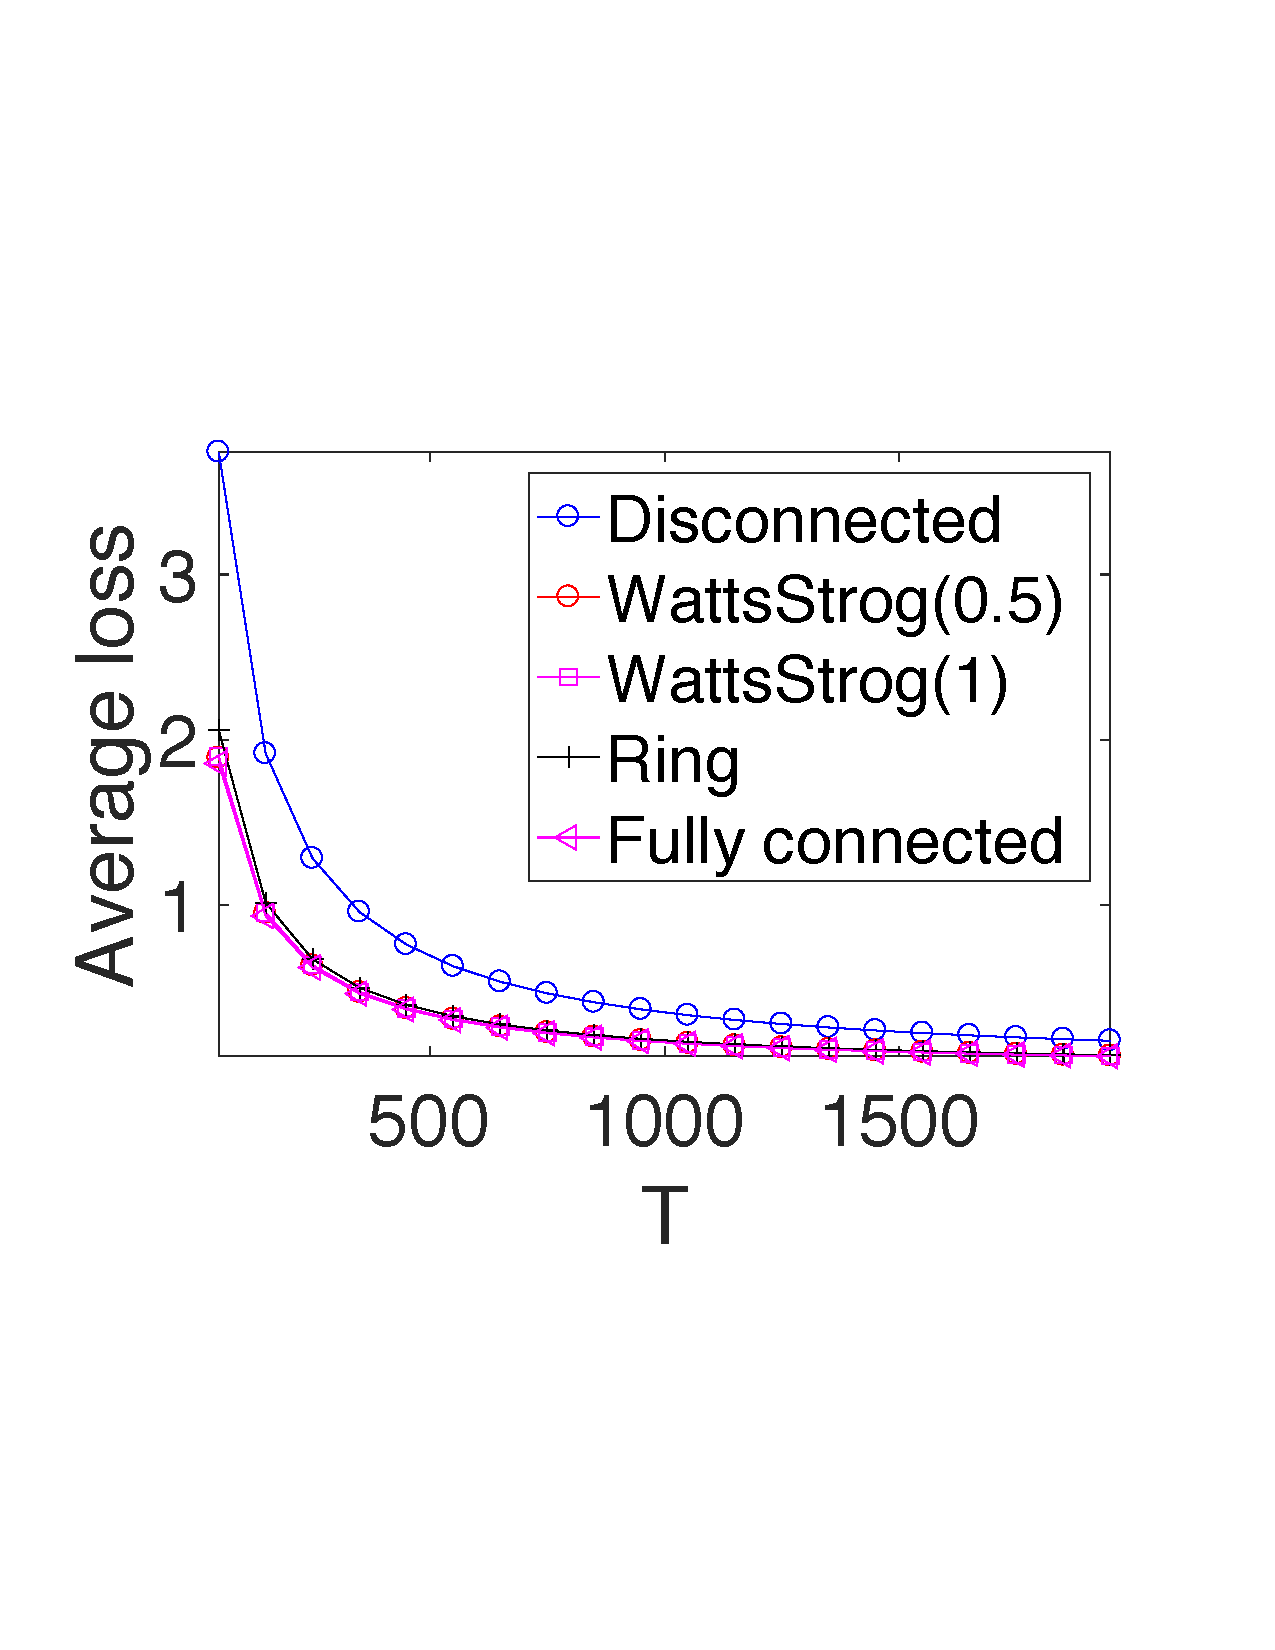
\includegraphics[width=0.48\columnwidth]{figure_ave_loss_topology_synthetic}\label{figure_ave_loss_topology_synthetic}}
\subfigure[\textit{room-occupancy}, $20$ nodes]{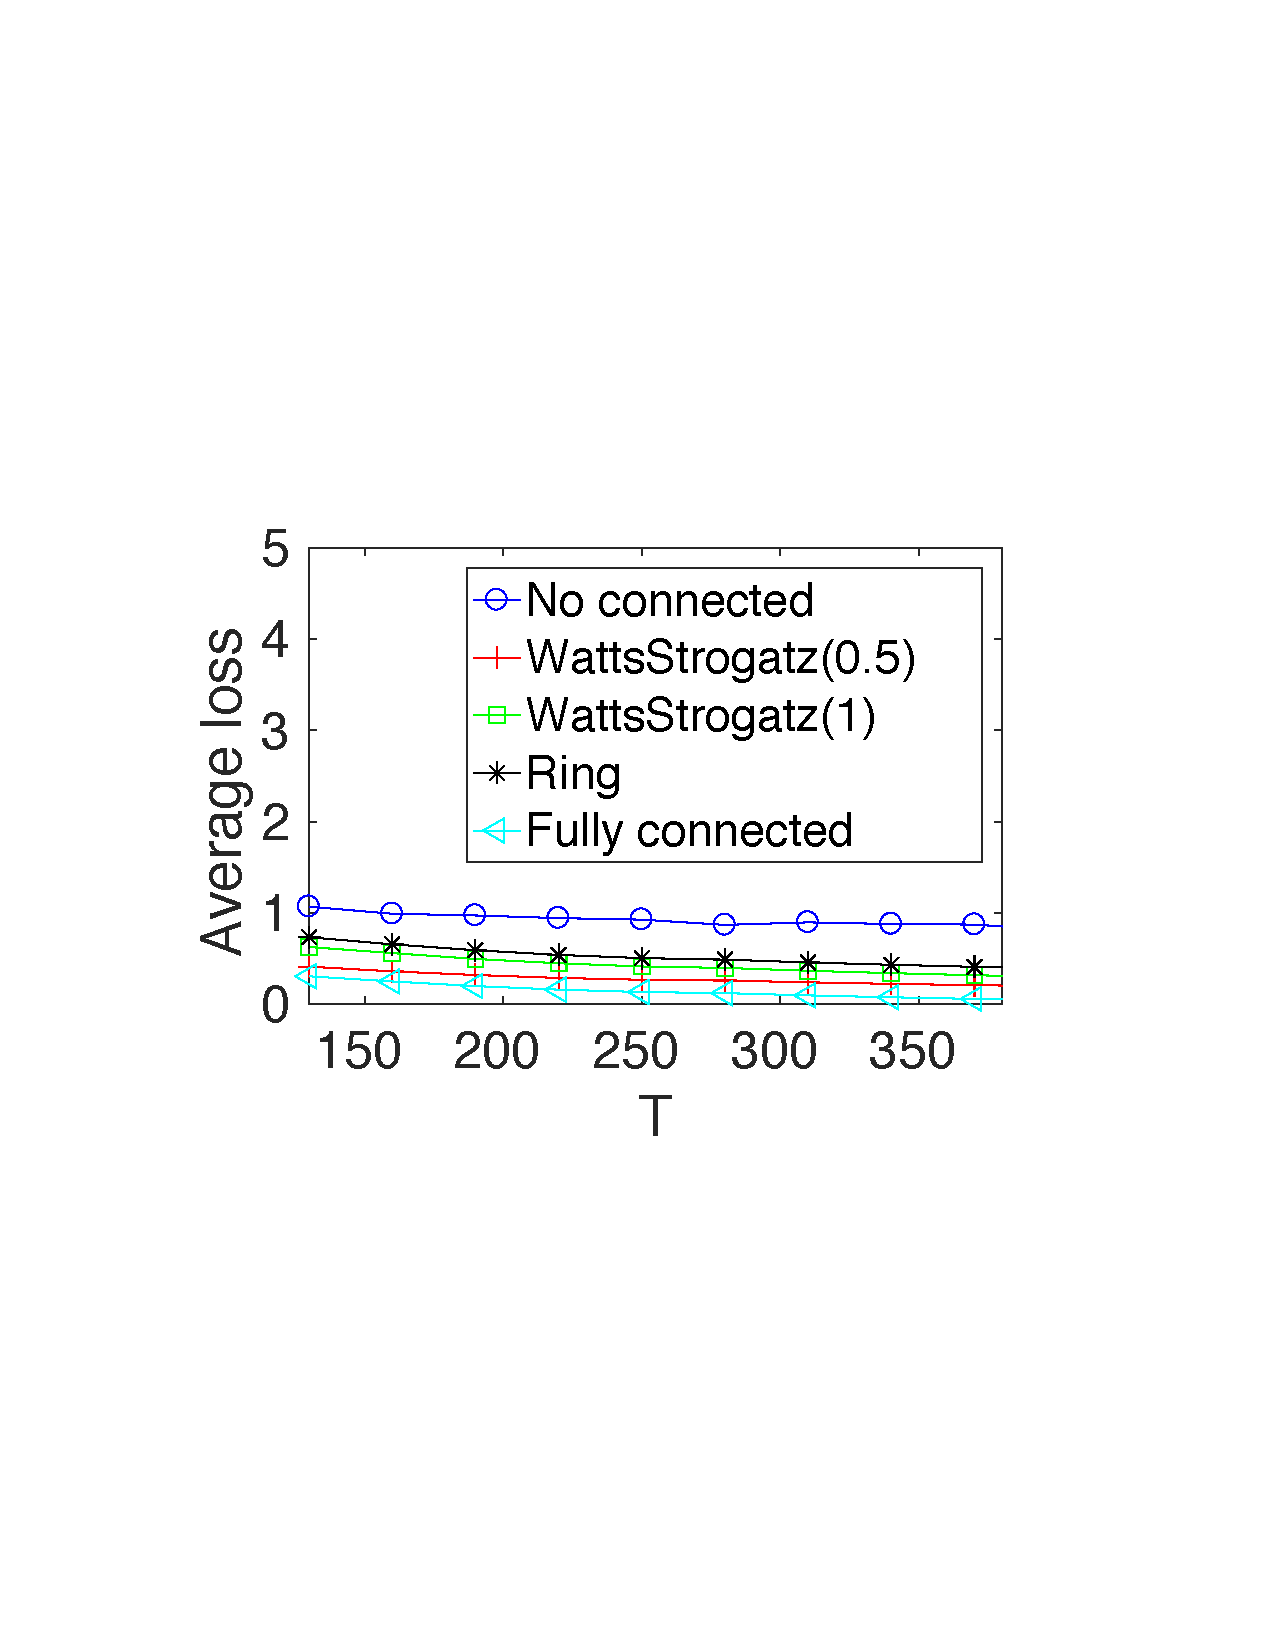
\includegraphics[width=0.48\columnwidth]{figure_ave_loss_topology_occupancy}\label{figure_ave_loss_topology_occupancy}}
\subfigure[\textit{usenet2}, $20$ nodes]{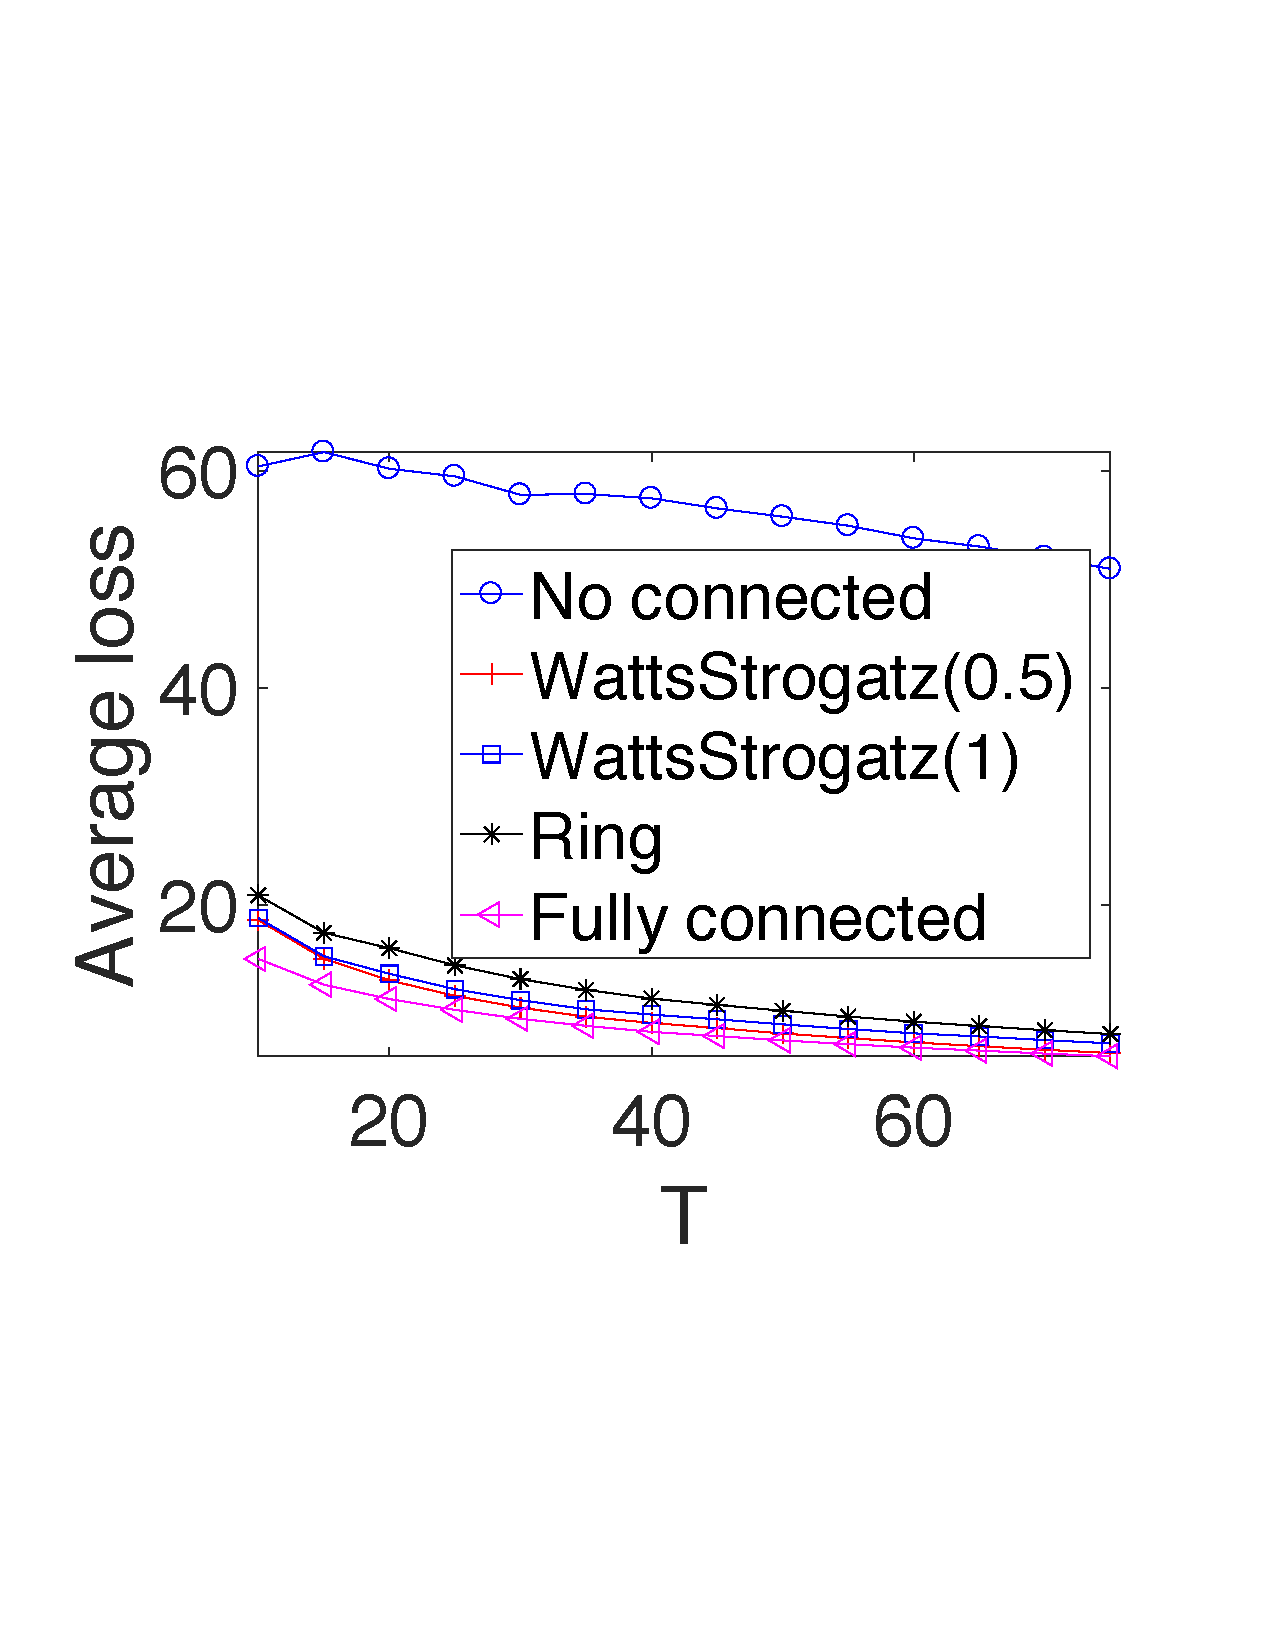
\includegraphics[width=0.48\columnwidth]{figure_ave_loss_topology_usenet2}\label{figure_ave_loss_topology_occupancy}}
\subfigure[\textit{spam}, $20$ nodes]{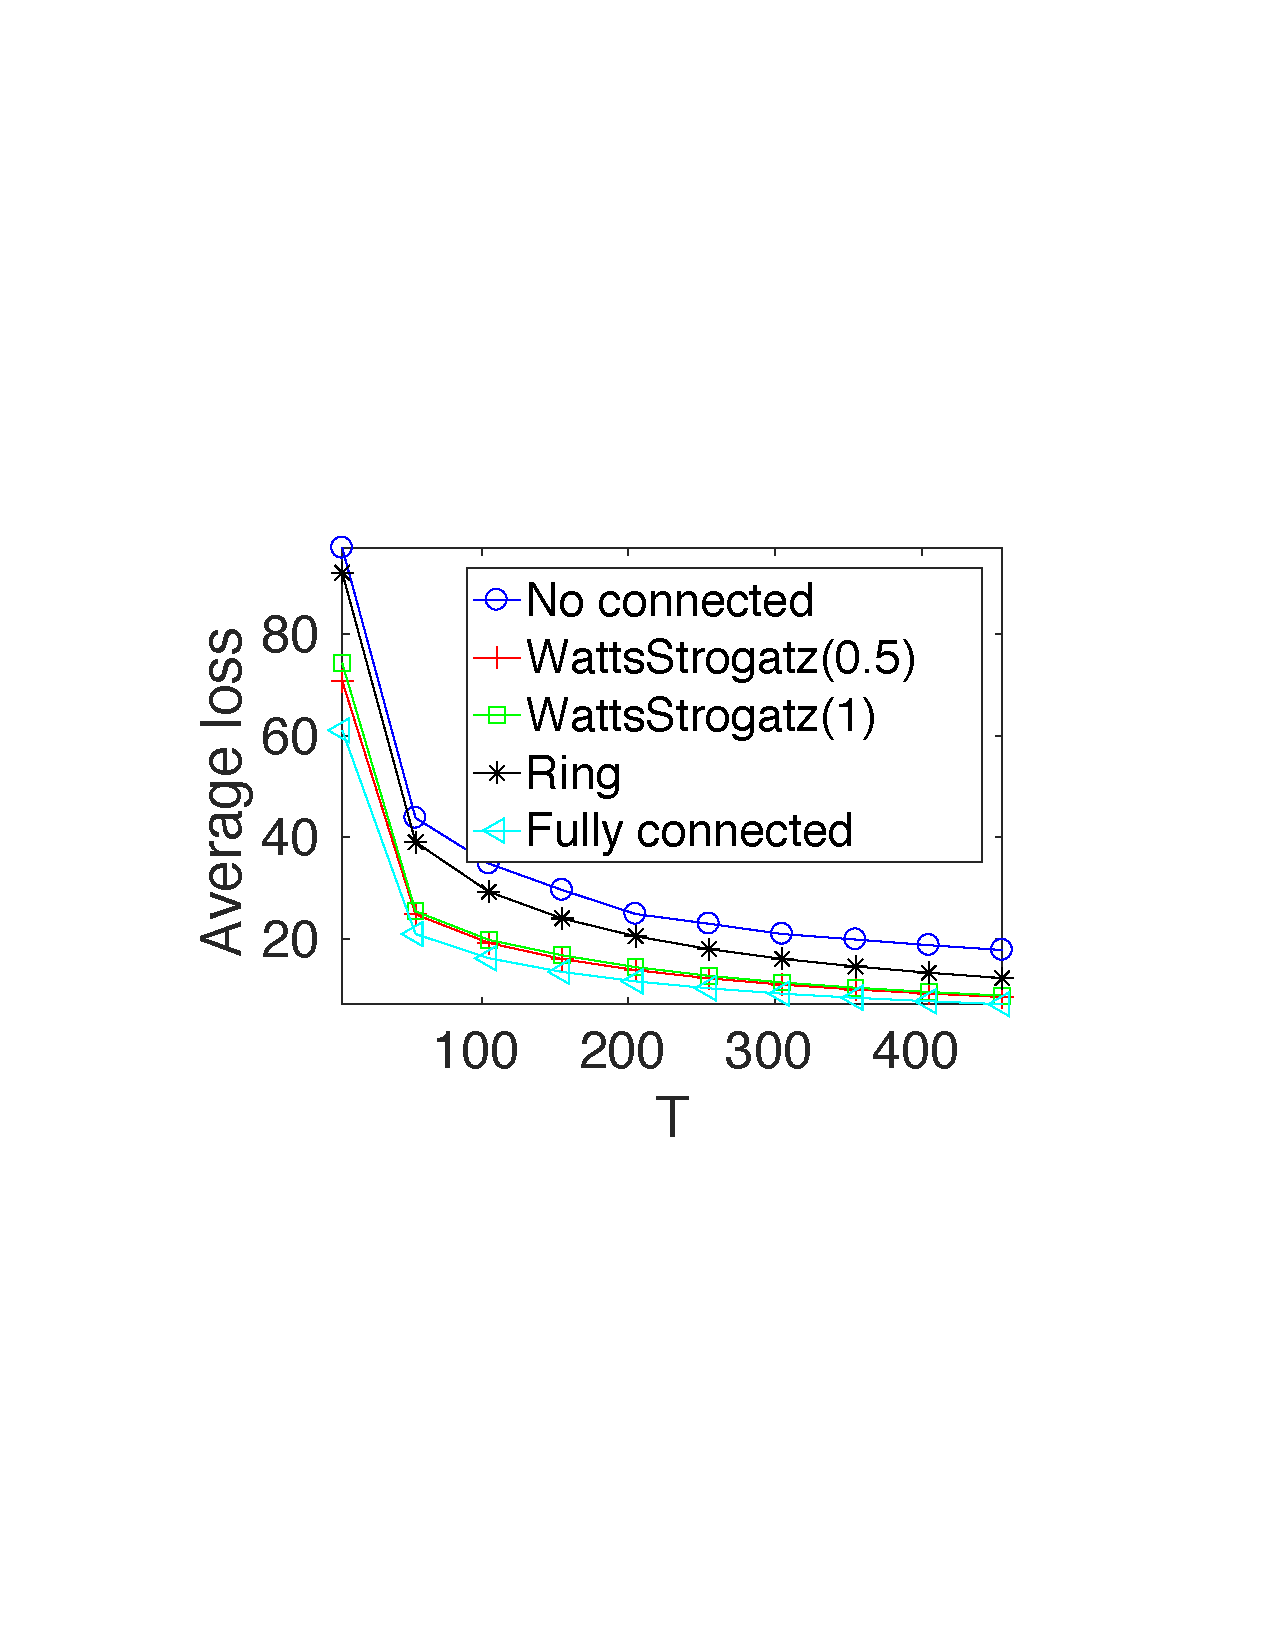
\includegraphics[width=0.48\columnwidth]{figure_ave_loss_topology_spam}\label{figure_ave_loss_topology_spam}}
\caption{The average loss yielded by DOG is insensitive to the topology of the network.}
\label{figure_compare_topology}
\end{figure*}



\section{Conclusion}
We investigate the online learning problem in a decentralized network, where the loss is incurred by both adversary and stochastic components.  We define a new dynamic regret, and propose a decentralized online gradient method. By using the new analysis framework, the decentralized online gradient method  achieves $\Ocal{n\sqrt{TM} + \sqrt{nT}\sigma}$ regret. It shows that the communication is only effective to decrease the regret caused by the stochastic loss. Extensive empirical studies validates the theoretical results. 


%\section*{References}
\bibliography{reference}

\bibliographystyle{abbrvnat}

\onecolumn

\section*{Appendix}

\textbf{Proof to Theorem \ref{theorem_regret_upper_bound}:}
\begin{proof}
From the regret definition, we have
\begin{align}
\nonumber
& \EE_{ \Xi_{n,t} \sim \Dcal_{n,t} } \frac{1}{n}\sum_{i=1}^n f_{i,t}(\x_{i,t};\xi_{i,t}) - f_{i,t}(\x_t^\ast;\xi_{i,t}) \\ \nonumber
\le & \EE_{ \Xi_{n,t} \sim \Dcal_{n,t} } \frac{1}{n}\sum_{i=1}^n \lrangle{ \nabla f_{i,t}(\x_{i,t};\xi_{i,t}),  \x_{i,t} - \x_t^\ast } \\ \nonumber
= & \underbrace{ \EE_{ \Xi_{n,t} \sim \Dcal_{n,t} } \frac{1}{n}\sum_{i=1}^n   \lrincir{\lrangle{\nabla  f_{i,t}(\x_{i,t};\xi_{i,t}), \x_{i,t} - \bar{\x}_t } + \lrangle{\nabla  f_{i,t}(\x_{i,t};\xi_{i,t}), \bar{\x}_t - \bar{\x}_{t+1} } } }_{I_1(t)} \\ \nonumber 
&+ \underbrace{ \EE_{ \Xi_{n,t} \sim \Dcal_{n,t} } \lrangle{\frac{1}{n}\sum_{i=1}^n\nabla f_{i,t}(\x_{i,t};\xi_{i,t}), \bar{\x}_{t+1} - \x_t^\ast } }_{I_2(t)}. \nonumber
\end{align}

Now, we begin to bound $I_1(t)$.
\begin{align}
\nonumber
I_1(t) = &    \lrincir{\underbrace{ \EE_{ \Xi_{n,t} \sim \Dcal_{n,t} }\frac{1}{n}\sum_{i=1}^n\lrangle{\nabla f_{i,t}(\x_{i,t}; \xi_{i,t}), \x_{i,t} - \bar{\x}_t } }_{J_1(t)} +  \underbrace{ \EE_{ \Xi_{n,t} \sim \Dcal_{n,t} }\lrangle{\frac{1}{n}\sum_{i=1}^n \nabla f_{i,t}(\x_{i,t};\xi_{i,t}), \bar{\x}_t - \bar{\x}_{t+1} }}_{J_2(t)}}.
\end{align} For $J_1(t)$, we have
\begin{align}
\nonumber
& J_1(t) \\ \nonumber 
= & \frac{1}{n}\EE_{ \Xi_{n,t} \sim \Dcal_{n,t} }\sum_{i=1}^n\lrangle{\nabla f_{i,t}(\x_{i,t}; \xi_{i,t}), \x_{i,t} - \bar{\x}_t } \\ \nonumber
= & \frac{1}{n}\EE_{ \Xi_{n,t} \sim \Dcal_{n,t} } \sum_{i=1}^n\lrangle{\nabla f_{i,t}(\x_{i,t}; \xi_{i,t}) - \nabla F_{i,t}(\bar{\x}_t), \x_{i,t} - \bar{\x}_t } + \frac{1}{n}\EE_{ \Xi_{n,t-1} \sim \Dcal_{t-1} }\sum_{i=1}^n\lrangle{\nabla F_{i,t}(\bar{\x}_t), \x_{i,t} - \bar{\x}_t } \\ \nonumber
= & \frac{1}{n}\EE_{ \Xi_{n,t-1} \sim \Dcal_{t-1} }\sum_{i=1}^n\lrangle{\nabla F_{i,t}(\x_{i,t}) - \nabla F_{i,t}(\bar{\x}_t), \x_{i,t} - \bar{\x}_t } + \EE_{ \Xi_{n,t-1} \sim \Dcal_{t-1} }\lrangle{\nabla F_{i,t}(\bar{\x}_t), \frac{1}{n}\sum_{i=1}^n\x_{i,t} - \bar{\x}_t } \\ \nonumber
\refabovecir{\le}{\textcircled{1}} & \frac{L}{n}\EE_{ \Xi_{n,t-1} \sim \Dcal_{t-1} }\sum_{i=1}^n \lrnorm{\x_{i,t} - \bar{\x}_t}^2. 
\end{align} $\textcircled{1}$ holds due to $F_{i,t}$ has $L$-Lipschitz gradients, and $\bar{\x}_t = \frac{1}{n}\sum_{i=1}^n \x_{i,t}$.

For $J_2(t)$, we have
\begin{align}
\nonumber
& J_2(t) \\ \nonumber 
= & \EE_{ \Xi_{n,t} \sim \Dcal_{n,t} }\lrangle{\frac{1}{n}\sum_{i=1}^n\nabla f_{i,t}(\x_{i,t};\xi_{i,t}), \bar{\x}_t - \bar{\x}_{t+1} } \\ \nonumber
\le & \frac{\eta}{2}\EE_{ \Xi_{n,t} \sim \Dcal_{n,t} } \lrnorm{\frac{1}{n}\sum_{i=1}^n \nabla f_{i,t}(\x_{i,t};\xi_{i,t})}^2 + \frac{1}{2\eta} \EE_{ \Xi_{n,t} \sim \Dcal_{n,t} }\lrnorm{ \bar{\x}_t - \bar{\x}_{t+1}}^2  \\ \nonumber
\le & \frac{\eta}{2}\EE_{ \Xi_{n,t} \sim \Dcal_{n,t} }\lrnorm{\frac{1}{n}\sum_{i=1}^n \lrincir{\nabla  f_{i,t}(\x_{i,t};\xi_{i,t}) - \nabla F_{i,t}(\x_{i,t}) + \nabla F_{i,t}(\x_{i,t})} }^2 + \frac{1}{2\eta} \EE_{ \Xi_{n,t} \sim \Dcal_{n,t} }\lrnorm{ \bar{\x}_t - \bar{\x}_{t+1}}^2  \\ \nonumber
\le &  \eta\EE_{ \Xi_{n,t} \sim \Dcal_{n,t} }\lrnorm{\frac{1}{n}\sum_{i=1}^n \lrincir{ \nabla f_{i,t}(\x_{i,t};\xi_{i,t}) - \nabla F_{i,t}(\x_{i,t}) } }^2 + \eta \EE_{ \Xi_{n,t-1} \sim \Dcal_{t-1} }\lrnorm{\frac{1}{n}\sum_{i=1}^n\nabla F_{i,t}(\x_{i,t})}^2 \\ \nonumber 
& + \frac{1}{2\eta} \EE_{ \Xi_{n,t} \sim \Dcal_{n,t} }\lrnorm{ \bar{\x}_t - \bar{\x}_{t+1}}^2  \\ \nonumber
\refabovecir{\le}{\textcircled{1}} & \frac{\eta}{n} \sigma^2 + \eta \EE_{ \Xi_{n,t-1} \sim \Dcal_{t-1} }\lrnorm{ \frac{1}{n}\sum_{i=1}^n \lrincir{ \nabla F_{i,t}(\x_{i,t}) - \nabla F_{i,t}(\bar{\x}_t) + \nabla F_{i,t}(\bar{\x}_t) } }^2 + \frac{1}{2\eta} \EE_{ \Xi_{n,t} \sim \Dcal_{n,t} }\lrnorm{ \bar{\x}_t - \bar{\x}_{t+1}}^2 \\ \nonumber
\le & \frac{\eta}{n} \sigma^2 + 2\eta \EE_{ \Xi_{n,t-1} \sim \Dcal_{t-1} }\lrnorm{\frac{1}{n}\sum_{i=1}^n \lrincir{ \nabla F_{i,t}(\x_{i,t}) - \nabla F_{i,t}(\bar{\x}_t) } }^2 \\ \nonumber 
& + 2\eta \EE_{ \Xi_{n,t-1} \sim \Dcal_{t-1} }\lrnorm{\nabla F_{i,t}(\bar{\x}_t)}^2 + \frac{1}{2\eta} \EE_{ \Xi_{n,t} \sim \Dcal_{n,t} }\lrnorm{ \bar{\x}_t - \bar{\x}_{t+1}}^2 \\ \nonumber
\le & \frac{\eta}{n} \sigma^2 + \frac{2\eta}{n} \EE_{ \Xi_{n,t-1} \sim \Dcal_{t-1} }\sum_{i=1}^n\lrnorm{ \nabla F_{i,t}(\x_{i,t}) - \nabla F_{i,t}(\bar{\x}_t)  }^2 \\ \nonumber 
& + 2\eta \EE_{ \Xi_{n,t-1} \sim \Dcal_{t-1} }\lrnorm{\nabla F_{i,t}(\bar{\x}_t)}^2 + \frac{1}{2\eta} \EE_{ \Xi_{n,t} \sim \Dcal_{n,t} }\lrnorm{ \bar{\x}_t - \bar{\x}_{t+1}}^2 \\ \nonumber
\refabovecir{\le}{\textcircled{2}} & \frac{\eta}{n} \sigma^2 + \frac{2\eta L^2}{n}\EE_{ \Xi_{n,t-1} \sim \Dcal_{t-1} }\sum_{i=1}^n \lrnorm{\x_{i,t} - \bar{\x}_t }^2 + 2\eta \EE_{ \Xi_{n,t-1} \sim \Dcal_{t-1} }\lrnorm{\nabla F_{i,t}(\bar{\x}_t)}^2 + \frac{1}{2\eta} \EE_{ \Xi_{n,t} \sim \Dcal_{n,t} }\lrnorm{ \bar{\x}_t - \bar{\x}_{t+1}}^2.
\end{align} $\textcircled{1}$ holds due to
\begin{align}
\nonumber
& \EE_{ \Xi_{n,t} \sim \Dcal_{n,t} }\lrnorm{\frac{1}{n}\sum_{i=1}^n \lrincir{ \nabla f_{i,t}(\x_{i,t};\xi_{i,t}) - \nabla F_{i,t}(\x_{i,t}) } }^2 \\ \nonumber
= & \frac{1}{n^2}\EE_{ \Xi_{n,t-1} \sim \Dcal_{t-1} }\lrincir{ \sum_{i=1}^n \EE_{ \xi_{i,t} \sim D_{i,t} }\lrnorm{ \nabla f_{i,t}(\x_{i,t};\xi_{i,t}) - \nabla F_{i,t}(\x_{i,t}) }^2  } \\ \nonumber 
& + \frac{1}{n^2}\EE_{ \Xi_{n,t-1} \sim \Dcal_{t-1} }\lrincir{2\sum_{i=1}^n\sum_{j=1, j\neq i}^n\lrangle{ \EE_{ \xi_{i,t} \sim D_{i,t} }\nabla f_{i,t}(\x_{i,t};\xi_{i,t}) - \nabla F_{i,t}(\x_{i,t}),  \EE_{ \xi_{j,t} \sim D_{j,t} } \nabla f_{i,t}(\x_{j,t};\xi_{j,t}) - \nabla F_{j,t}(\x_{j,t})} } \\ \nonumber
= & \frac{1}{n^2}\EE_{ \Xi_{n,t-1} \sim \Dcal_{t-1} }\sum_{i=1}^n \EE_{ \xi_{i,t} \sim D_{i,t} }\lrnorm{ \nabla f_{i,t}(\x_{i,t};\xi_{i,t}) - \nabla F_{i,t}(\x_{i,t}) }^2 + 0 \\ \nonumber
\le & \frac{1}{n} \sigma^2.
\end{align} $\textcircled{2}$ holds due to $F_{i,t}$ has $L$ Lipschitz gradients.

 Therefore, we obtain
\begin{align}
\nonumber
& I_1(t) \\ \nonumber 
= &  (J_1(t) + J_2(t)) \\ \nonumber
= &   \lrincir{ \frac{L}{n}\EE_{ \Xi_{n,t-1} \sim \Dcal_{t-1} }\sum_{i=1}^n \lrnorm{\x_{i,t} - \bar{\x}_t}^2 +\frac{\eta}{n} \sigma^2 + \frac{2\eta L^2}{n}\EE_{ \Xi_{n,t-1} \sim \Dcal_{t-1} }\sum_{i=1}^n \lrnorm{\x_{i,t} - \bar{\x}_t }^2 } \\ \nonumber
& +  \lrincir{ 2\eta \EE_{ \Xi_{n,t-1} \sim \Dcal_{t-1} }\lrnorm{\nabla F_{i,t}(\bar{\x}_t)}^2 + \frac{1}{2\eta} \EE_{ \Xi_{n,t} \sim \Dcal_{n,t} }\lrnorm{ \bar{\x}_t - \bar{\x}_{t+1}}^2 } \\ \nonumber
\le &   \lrincir{ \frac{L}{n} + \frac{2\eta L^2}{n} }\EE_{ \Xi_{n,t-1} \sim \Dcal_{t-1} }\sum_{i=1}^n\lrnorm{\x_{i,t} - \bar{\x}_t }^2   + 2\eta  \EE_{ \Xi_{n,t-1} \sim \Dcal_{t-1} }\lrnorm{\nabla F_{i,t}(\bar{\x}_t)}^2 \\ \nonumber 
&+ \frac{\eta  \sigma^2}{n} +  \frac{1}{2\eta} \EE_{ \Xi_{n,t} \sim \Dcal_{n,t} }\lrnorm{ \bar{\x}_t - \bar{\x}_{t+1}}^2.
\end{align}

Therefore, we have 
\begin{align}
\nonumber
\sum_{t=1}^T I_1(t) \le &  \lrincir{ \frac{L}{n} + \frac{2\eta L^2}{n} }\EE_{ \Xi_{n,t-1} \sim \Dcal_{t-1} }\sum_{i=1}^n\sum_{t=1}^T\lrnorm{\x_{i,t} - \bar{\x}_t }^2   + 2\eta  \EE_{ \Xi_{n,t-1} \sim \Dcal_{t-1} }\sum_{t=1}^T\lrnorm{\nabla F_{i,t}(\bar{\x}_t)}^2 \\ \nonumber 
&+ \frac{T\eta  \sigma^2}{n} +  \frac{1}{2\eta} \EE_{ \Xi_{n,t} \sim \Dcal_{n,t} }\sum_{t=1}^T\lrnorm{ \bar{\x}_t - \bar{\x}_{t+1}}^2.
\end{align} 




Now, we begin to bound $I_2(t)$. Recall that the update rule is 
\begin{align}
\nonumber
\x_{i,t+1} = \sum_{j=1}^n \W_{ij}\x_{j,t} - \eta \nabla f_{i,t}(\x_{i,t};\xi_{i,t}).
\end{align}  According to Lemma \ref{Lemma_average_update_rule}, we have 
\begin{align}
\label{equa_thoerem_update_rule_equivalent}
\bar{\x}_{t+1} = \bar{\x}_t - \eta \lrincir{\frac{1}{n}\sum_{i=1}^n \nabla f_{i,t}(\x_{i,t};\xi_{i,t})}.
\end{align} 
Denote a new auxiliary function $\phi(\z)$ as 
\begin{align}
\nonumber
\phi(\z) = \lrangle{\frac{1}{n}\sum_{i=1}^n \nabla f_{i,t}(\x_{i,t};\xi_{i,t}), \z} + \frac{1}{2\eta}\lrnorm{\z - \bar{\x}_t}^2.
\end{align} 

It is trivial to verify that \eqref{equa_thoerem_update_rule_equivalent} satisfies the first-order optimality condition of the optimization problem: $\min_{\z\in\RR^d} \phi(\z)$, that is,
\begin{align}
\nonumber
\nabla \phi(\bar{\x}_{t+1}) = \0.
\end{align} We thus have 
\begin{align}
\nonumber
\bar{\x}_{t+1} = & \argmin_{\z\in\RR^d} \phi(\z) \\ \nonumber
= & \argmin_{\z\in\RR^d} \lrangle{\frac{1}{n}\sum_{i=1}^n \nabla f_{i,t}(\x_{i,t};\xi_{i,t}), \z} + \frac{1}{2\eta}\lrnorm{\z - \bar{\x}_t}^2.
\end{align} Furthermore, denote a new auxiliary variable $\bar{\x}_{\tau}$ as  
\begin{align}
\nonumber
\bar{\x}_{\tau} = \bar{\x}_{t+1} + \tau \lrincir{\x_t^\ast - \bar{\x}_{t+1}},
\end{align} where $0< \tau \le 1$. According to the optimality of $\bar{\x}_{t+1}$, we have
\begin{align}
\nonumber
0 \le & \phi(\bar{\x}_{\tau}) - \phi(\bar{\x}_{t+1}) \\ \nonumber
= & \lrangle{\frac{1}{n}\sum_{i=1}^n \nabla f_{i,t}(\x_{i,t};\xi_{i,t}), \bar{\x}_{\tau} - \bar{\x}_{t+1}} + \frac{1}{2\eta}\lrincir{ \lrnorm{\bar{\x}_{\tau} - \bar{\x}_t}^2 - \lrnorm{\bar{\x}_{t+1} - \bar{\x}_t}^2 } \\ \nonumber
= & \lrangle{\frac{1}{n}\sum_{i=1}^n \nabla f_{i,t}(\x_{i,t};\xi_{i,t}), \tau \lrincir{\x_t^\ast - \bar{\x}_{t+1}}} + \frac{1}{2\eta}\lrincir{ \lrnorm{\bar{\x}_{t+1} + \tau \lrincir{\x_t^\ast - \bar{\x}_{t+1}} - \bar{\x}_t}^2 - \lrnorm{\bar{\x}_{t+1} - \bar{\x}_t}^2 } \\ \nonumber
= & \lrangle{\frac{1}{n}\sum_{i=1}^n \nabla f_{i,t}(\x_{i,t};\xi_{i,t}), \tau \lrincir{\x_t^\ast - \bar{\x}_{t+1}}} + \frac{1}{2\eta}\lrincir{ \lrnorm{\tau \lrincir{\x_t^\ast - \bar{\x}_{t+1}}}^2 + 2\lrangle{\tau \lrincir{\x_t^\ast - \bar{\x}_{t+1}}, \bar{\x}_{t+1} - \bar{\x}_t } }.
\end{align} Note that the above inequality holds for any $0< \tau \le 1$. Divide $\tau$ on both sides, and we have
\begin{align}
\nonumber
I_2(t) = & \EE_{ \Xi_{n,t} \sim \Dcal_{n,t} } \lrangle{\frac{1}{n}\sum_{i=1}^n \nabla f_{i,t}(\x_{i,t};\xi_{i,t}), \bar{\x}_{t+1} - \x_t^\ast} \\ \nonumber 
\le & \frac{1}{2\eta}\EE_{ \Xi_{n,t} \sim \Dcal_{n,t} }\lrincir{ \lim_{\tau \rightarrow 0^+}\tau \lrnorm{\lrincir{\x_t^\ast - \bar{\x}_{t+1}}}^2 + 2\lrangle{ \x_t^\ast - \bar{\x}_{t+1}, \bar{\x}_{t+1} - \bar{\x}_t } } \\ \nonumber
= & \frac{1}{\eta}\EE_{ \Xi_{n,t} \sim \Dcal_{n,t} }\lrangle{ \x_t^\ast - \bar{\x}_{t+1}, \bar{\x}_{t+1} - \bar{\x}_t } \\ \label{equa_I3_temp}
= & \frac{1}{2\eta}\EE_{ \Xi_{n,t} \sim \Dcal_{n,t} }\lrincir{ \lrnorm{\x_t^\ast - \bar{\x}_t}^2 - \lrnorm{\x_t^\ast - \bar{\x}_{t+1}}^2 - \lrnorm{\bar{\x}_t - \bar{\x}_{t+1}}^2 }. 
\end{align} Besides, we have
\begin{align}
\nonumber
& \lrnorm{\x_{t+1}^\ast - \bar{\x}_{t+1}}^2 - \lrnorm{\x_t^\ast - \bar{\x}_{t+1}}^2 \\ \nonumber 
= & \lrnorm{\x_{t+1}^\ast}^2 - \lrnorm{\x_t^\ast}^2 - 2\lrangle{\bar{\x}_{t+1}, -\x_t^\ast + \x_{t+1}^\ast} \\ \nonumber
= & \lrincir{\lrnorm{\x_{t+1}^\ast} - \lrnorm{\x_t^\ast}} \lrincir{\lrnorm{\x_{t+1}^\ast} + \lrnorm{\x_t^\ast}} - 2\lrangle{\bar{\x}_{t+1}, -\x_t^\ast + \x_{t+1}^\ast} \\ \nonumber
\le & \lrnorm{\x_{t+1}^\ast - \x_t^\ast} \lrincir{\lrnorm{\x_{t+1}^\ast} + \lrnorm{\x_t^\ast}} + 2\lrnorm{\bar{\x}_{t+1}} \lrnorm{\x_{t+1}^\ast-\x_t^\ast} \\ \nonumber
\le & 4\sqrt{R}\lrnorm{\x_{t+1}^\ast - \x_t^\ast}.   
\end{align} The last inequality holds due to our assumption, that is, $\lrnorm{\x_{t+1}^\ast}=\lrnorm{\x_{t+1}^\ast - \0}\le \sqrt{R}$, $\lrnorm{\x_t^\ast} = \lrnorm{\x_t^\ast-\0} \le \sqrt{R}$, and $\lrnorm{\bar{\x}_{t+1}} = \lrnorm{\bar{\x}_{t+1}-\0} \le \sqrt{R}$. 

Thus, telescoping $I_2(t)$ over $t\in[T]$, we have 
\begin{align}
\nonumber
\sum_{t=1}^T I_2(t) \le & \frac{1}{2\eta}\EE_{ \Xi_{n,T} \sim \Dcal_{n,T} }\lrincir{ 4\sqrt{R}\sum_{t=1}^T\lrnorm{\x_{t+1}^\ast - \x_t^\ast} + \lrnorm{\bar{\x}_1^\ast - \bar{\x}_1}^2 - \lrnorm{\bar{\x}_T^\ast - \bar{\x}_{T+1}}^2 } - \frac{1}{2\eta} \EE_{ \Xi_{n,T} \sim \Dcal_{n,T} }\sum_{t=1}^T \lrnorm{\bar{\x}_t - \bar{\x}_{t+1}}^2 \\ \nonumber
\le & \frac{1}{2\eta}\lrincir{ 4\sqrt{R} M + R } - \frac{1}{2\eta} \EE_{ \Xi_{n,T} \sim \Dcal_{n,T} } \sum_{t=1}^T \lrnorm{\bar{\x}_t - \bar{\x}_{t+1} }^2.
\end{align} Here, $M$ the budget of the dynamics, which is defined in \eqref{equa_define_M}.

 
Combining those bounds of $I_1(t)$, and $I_2(t)$ together, we finally obtain
\begin{align}
\nonumber
& \EE_{ \Xi_{n,T} \sim \Dcal_{n,T} } \sum_{t=1}^T\sum_{i=1}^n f_{i,t}(\x_{i,t};\xi_{i,t}) - f_{i,t}(\x_t^\ast;\xi_{i,t}) \\ \nonumber
\le & n \sum_{t=1}^T \lrincir{ I_1(t) + I_2(t) } \\ \nonumber
\le & \lrincir{ \frac{L}{n} + \frac{2\eta L^2}{n} }\EE_{ \Xi_{n,t-1} \sim \Dcal_{t-1} }\sum_{i=1}^n\sum_{t=1}^T\lrnorm{\x_{i,t} - \bar{\x}_t }^2   + 2\eta  \EE_{ \Xi_{n,t-1} \sim \Dcal_{t-1} }\sum_{t=1}^T\lrnorm{\nabla F_{i,t}(\bar{\x}_t)}^2 + \frac{T\eta  \sigma^2}{n}   + \frac{n}{2\eta}\lrincir{ 4\sqrt{R}M + R  } \\ \nonumber
\refabovecir{\le}{\textcircled{1}} & \eta T \sigma^2 + 4n \EE_{ \Xi_{n,T} \sim \Dcal_{n,T} } \sum_{t=1}^T  \lrincir{F_{i,t}(\bar{\x}_t) - F_{i,t}(\bar{\x}_{t+1})}  +  \lrincir{L + 2\eta L^2  + 4L^2 \eta}  \EE_{ \Xi_{n,T} \sim \Dcal_{n,T} }\sum_{t=1}^T\sum_{i=1}^n \lrnorm{ \bar{\x}_t - \x_{i,t} }^2  \\ \nonumber
& + 4n \lrincir{ 4T  \eta G^2 + \frac{TG^2L\eta^2}{2} }  + \frac{n}{2\eta}\lrincir{ 4\sqrt{R}M + R  }\\ \nonumber
\refabovecir{\le}{\textcircled{2}} & \eta T \sigma^2 + 4n \EE_{ \Xi_{n,T} \sim \Dcal_{n,T} } \sum_{t=1}^T  \lrincir{F_{i,t}(\bar{\x}_t) - F_{i,t}(\bar{\x}_{t+1})}  +  \lrincir{ L + 2\eta L^2  + 4L^2 \eta}  \frac{nT\eta^2 G^2 }{(1-\rho)^2}  \\ \nonumber
& + 4n \lrincir{ 4T  \eta G^2 + \frac{TG^2L\eta^2}{2} }  + \frac{n}{2\eta}\lrincir{ 4\sqrt{R}M + R  } \\ \nonumber
\refabovecir{\le}{\textcircled{3}} & \eta T \sigma^2 + 4n  T\eta G^2  + \lrincir{ L + 2\eta L^2  + 4L^2 \eta}  \frac{nT\eta^2 G^2 }{(1-\rho)^2}  + 4n\lrincir{ 4T  \eta G^2 + \frac{TG^2L\eta^2}{2} }  + \frac{n}{2\eta}\lrincir{ 4\sqrt{R}M + R  }.
\end{align}  
$\textcircled{1}$ holds due to Lemma \ref{Lemma_gradient_norm_bound}. That is, we have
\begin{align}
\nonumber
& \frac{\eta}{2} \EE_{ \Xi_{n,T-1} \sim \Dcal_{n,T-1} }\sum_{t=1}^T \lrnorm{\nabla F_{i,t}(\bar{\x}_t)}^2 \\ \nonumber
\le & \EE_{ \Xi_{n,T} \sim \Dcal_{n,T} } \sum_{t=1}^T  \lrincir{F_{i,t}(\bar{\x}_t) - F_{i,t}(\bar{\x}_{t+1})} + 4T  \eta G^2 + \frac{ L^2 \eta}{n}\EE_{ \Xi_{n,T-1} \sim \Dcal_{n,T-1} }\sum_{t=1}^T\sum_{i=1}^n \lrnorm{ \bar{\x}_t - \x_{i,t} }^2 + \frac{TG^2L\eta^2}{2}.
\end{align} $\textcircled{2}$ holds due to Lemma \ref{Lemma_x_variance_norm_square}
\begin{align}
\nonumber
\EE_{ \Xi_{n,T-1} \sim \Dcal_{n,T-1} } \sum_{i=1}^n\sum_{t=1}^T \lrnorm{\x_{i,t} - \bar{\x}_t}^2 \le \frac{nT\eta^2 G^2 }{(1-\rho)^2}.
\end{align} $\textcircled{3}$ holds due to 
\begin{align}
\nonumber
& \EE_{ \Xi_{n,t} \sim \Dcal_{n,t} } \lrincir{F_{i,t}(\bar{\x}_t) - F_{i,t}(\bar{\x}_{t+1}) } \\ \nonumber 
\le & \EE_{ \Xi_{n,t} \sim \Dcal_{n,t} } \lrangle{\nabla F_{i,t}(\bar{\x}_t), \bar{\x}_t - \bar{\x}_{t+1}} \\ \nonumber
= & \EE_{ \Xi_{n,t} \sim \Dcal_{n,t} } \lrangle{\nabla F_{i,t}(\bar{\x}_t), \frac{\eta}{n}\sum_{i=1}^n\nabla f_{i,t}(\x_{i,t};\xi_{i,t}) } \\ \nonumber
\le & \eta\EE_{ \Xi_{n,t} \sim \Dcal_{n,t} }\lrincir{ \frac{1}{2}\lrnorm{\nabla F_{i,t}(\bar{\x}_t)}^2 + \frac{1}{2} \lrnorm{\frac{1}{n}\sum_{i=1}^n\nabla f_{i,t}(\x_{i,t};\xi_{i,t})}^2 }\\ \nonumber
\le & \eta\EE_{ \Xi_{n,t} \sim \Dcal_{n,t} }\lrincir{ \frac{1}{2}\lrnorm{\nabla F_{i,t}(\bar{\x}_t)}^2 + \frac{1}{2n}\sum_{i=1}^n\lrnorm{\nabla f_{i,t}(\x_{i,t};\xi_{i,t})}^2 }\\ \nonumber
\le & \eta G^2. 
\end{align}

Re-arranging items, we have
\begin{align}
\nonumber
& \EE_{ \Xi_{n,T} \sim \Dcal_{n,T} } \sum_{t=1}^T\sum_{i=1}^n f_{i,t}(\x_{i,t};\xi_{i,t}) - f_{i,t}(\x_t^\ast;\xi_{i,t}) \\ \nonumber
\le & 20\eta T n G^2 +  \eta T\sigma^2 + \lrincir{\frac{L + 2\eta L^2  + 4L^2 \eta}{(1-\rho)^2} +2L}  nT\eta^2 G^2    + \frac{n}{2\eta}\lrincir{ 4\sqrt{R}M + R  }.
\end{align}

It completes the proof.



\end{proof}




\begin{Lemma}
\label{Lemma_gradient_norm_bound}
Using Assumption \ref{assumption_bounded_gradient_domain}, and setting $\eta>0$ in Algorithm \ref{algo_DOG}, we have 
\begin{align}
& \frac{\eta}{2} \EE_{ \Xi_{n,T-1} \sim \Dcal_{n,T-1} }\sum_{t=1}^T \lrnorm{\nabla F_{i,t}(\bar{\x}_t)}^2 \\ \nonumber
\le & \EE_{ \Xi_{n,T} \sim \Dcal_{n,T} } \sum_{t=1}^T  \lrincir{F_{i,t}(\bar{\x}_t) - F_{i,t}(\bar{\x}_{t+1})} + 4T  \eta G^2 + \frac{ L^2 \eta}{n}\EE_{ \Xi_{n,T-1} \sim \Dcal_{n,T-1} }\sum_{t=1}^T\sum_{i=1}^n \lrnorm{ \bar{\x}_t - \x_{i,t} }^2 + \frac{TG^2L\eta^2}{2}.
\end{align}
\end{Lemma}

\begin{proof}
We have
\begin{align}
\nonumber
& \EE_{ \Xi_{n,t} \sim \Dcal_{n,t} } F_{i,t}(\bar{\x}_{t+1}) \\ \nonumber
\le & \EE_{ \Xi_{n,t-1} \sim \Dcal_{t-1} } F_{i,t}(\bar{\x}_t) + \EE_{ \Xi_{n,t} \sim \Dcal_{n,t} }\lrangle{\nabla F_{i,t}(\bar{\x}_t), \bar{\x}_{t+1} - \bar{\x}_t} + \frac{L}{2}\EE_{ \Xi_{n,t} \sim \Dcal_{n,t} }\lrnorm{\bar{\x}_{t+1} - \bar{\x}_t}^2 \\ \nonumber
= & \EE_{ \Xi_{n,t-1} \sim \Dcal_{t-1} } F_{i,t}(\bar{\x}_t) + \EE_{ \Xi_{n,t} \sim \Dcal_{n,t} }\lrangle{\nabla F_{i,t}(\bar{\x}_t), -\frac{\eta}{n}\sum_{i=1}^n \nabla f_{i,t}(\x_{i,t};\xi_{i,t})} + \frac{L}{2} \EE_{ \Xi_{n,t} \sim \Dcal_{n,t} }\lrnorm{\frac{\eta}{n}\sum_{i=1}^n \nabla f_{i,t}(\x_{i,t};\xi_{i,t})}^2 \\ \label{equa_Lemma_gradient_norm_temp0}
= & \EE_{ \Xi_{n,t-1} \sim \Dcal_{t-1} } F_{i,t}(\bar{\x}_t) + \EE_{ \Xi_{n,t-1} \sim \Dcal_{t-1} }\lrangle{\nabla F_{i,t}(\bar{\x}_t), -\frac{\eta}{n}\sum_{i=1}^n \nabla f_{i,t}(\x_{i,t};\xi_{i,t})} + \frac{L}{2} \EE_{ \Xi_{n,t} \sim \Dcal_{n,t} }\lrnorm{\frac{\eta}{n}\sum_{i=1}^n \nabla f_{i,t}(\x_{i,t};\xi_{i,t})}^2.
\end{align}


Besides, we have
\begin{align}
\nonumber
& \EE_{ \Xi_{n,t-1} \sim \Dcal_{t-1} } \lrangle{\nabla F_{i,t}(\bar{\x}_t), -\frac{\eta}{n}\sum_{i=1}^n \nabla f_{i,t}(\x_{i,t};\xi_{i,t})} \\ \nonumber
= & \EE_{ \Xi_{n,t-1} \sim \Dcal_{t-1} } \frac{\eta}{2}\lrincir{ \lrnorm{\nabla F_{i,t}(\bar{\x}_t) -\frac{1}{n}\sum_{i=1}^n \nabla f_{i,t}(\x_{i,t};\xi_{i,t})}^2 - \lrnorm{\nabla F_{i,t}(\bar{\x}_t)}^2 - \lrnorm{\frac{1}{n}\sum_{i=1}^n \nabla f_{i,t}(\x_{i,t};\xi_{i,t})}^2 } \\ \nonumber
\le & \EE_{ \Xi_{n,t-1} \sim \Dcal_{t-1} } \frac{\eta}{2}\lrincir{ \lrnorm{\nabla F_{i,t}(\bar{\x}_t) -\frac{1}{n}\sum_{i=1}^n \lrincir{  \nabla  f_{i,t}(\x_{i,t};\xi_{i,t}) +   \nabla F_{i,t}(\x_{i,t}) } }^2 }  - \EE_{ \Xi_{n,t-1} \sim \Dcal_{t-1} } \frac{\eta}{2} \lrnorm{\nabla F_{i,t}(\bar{\x}_t)}^2  \\ \nonumber
\le & \EE_{ \Xi_{n,t-1} \sim \Dcal_{t-1} } \frac{\eta}{2}\lrincir{ 2 \lrnorm{\nabla F_{i,t}(\bar{\x}_t) -\frac{1}{n}\sum_{i=1}^n \nabla  f_{i,t}(\x_{i,t};\xi_{i,t})}^2 + 2 \lrnorm{ \nabla F_{i,t}(\bar{\x}_t) - \frac{1}{n}\sum_{i=1}^n\nabla F_{i,t}(\x_{i,t}) }^2 } \\ \nonumber 
& - \EE_{ \Xi_{n,t-1} \sim \Dcal_{t-1} } \frac{\eta}{2} \lrnorm{\nabla F_{i,t}(\bar{\x}_t)}^2  \\ \nonumber
\le & \EE_{ \Xi_{n,t-1} \sim \Dcal_{t-1} } \frac{\eta}{2}\lrincir{ 2 \lrnorm{\nabla F_{i,t}(\bar{\x}_t) -\frac{1}{n}\sum_{i=1}^n \nabla  f_{i,t}(\x_{i,t};\xi_{i,t})}^2 + \frac{2}{n}\sum_{i=1}^n \lrnorm{ \nabla F_{i,t}(\bar{\x}_t) - \nabla F_{i,t}(\x_{i,t}) }^2 } \\ \nonumber 
& - \EE_{ \Xi_{n,t-1} \sim \Dcal_{t-1} } \frac{\eta}{2} \lrnorm{\nabla F_{i,t}(\bar{\x}_t)}^2  \\ \nonumber
\le & \EE_{ \Xi_{n,t-1} \sim \Dcal_{t-1} } \frac{\eta}{2}\lrincir{ 2 \lrnorm{\nabla F_{i,t}(\bar{\x}_t) -\frac{1}{n}\sum_{i=1}^n \nabla  f_{i,t}(\x_{i,t};\xi_{i,t})}^2 + \frac{2L^2}{n}\sum_{i=1}^n \lrnorm{ \bar{\x}_t - \x_{i,t} }^2 }  - \EE_{ \Xi_{n,t-1} \sim \Dcal_{t-1} } \frac{\eta}{2} \lrnorm{\nabla F_{i,t}(\bar{\x}_t)}^2  \\ \nonumber
\le & \EE_{ \Xi_{n,t-1} \sim \Dcal_{t-1} } \frac{\eta}{2}\lrincir{ 4 \lrnorm{\nabla F_{i,t}(\bar{\x}_t)}^2  + 4 \lrnorm{\frac{1}{n}\sum_{i=1}^n \nabla  f_{i,t}(\x_{i,t};\xi_{i,t})}^2 + \frac{2L^2}{n}\sum_{i=1}^n \lrnorm{ \bar{\x}_t - \x_{i,t} }^2 }  - \EE_{ \Xi_{n,t-1} \sim \Dcal_{t-1} } \frac{\eta}{2} \lrnorm{\nabla F_{i,t}(\bar{\x}_t)}^2 \\ \label{equa_Lemma_gradient_norm_temp1}
\refabovecir{\le}{\textcircled{1}} & \EE_{ \Xi_{n,t-1} \sim \Dcal_{t-1} } \frac{\eta}{2}\lrincir{ 8 G^2 + \frac{2L^2}{n}\sum_{i=1}^n \lrnorm{ \bar{\x}_t - \x_{i,t} }^2 }  - \EE_{ \Xi_{n,t} \sim \Dcal_{n,t} } \frac{\eta}{2} \lrnorm{\nabla F_{i,t}(\bar{\x}_t)}^2.
\end{align} $\textcircled{1}$ holds due to  
\begin{align}
\nonumber
\EE_{ \Xi_{n,t-1} \sim \Dcal_{t-1} }\lrnorm{\frac{1}{n}\sum_{i=1}^n \nabla  f_{i,t}(\x_{i,t};\xi_{i,t})}^2 \le \frac{1}{n}\sum_{i=1}^n  \EE_{ \Xi_{n,t-1} \sim \Dcal_{t-1} }\lrnorm{\nabla  f_{i,t}(\x_{i,t};\xi_{i,t})}^2 \le G^2.
\end{align}

Recall that
\begin{align}
\label{equa_Lemma_gradient_norm_temp2}
\EE_{ \Xi_{n,t} \sim \Dcal_{n,t} }\lrnorm{ \nabla f_{i,t}(\x_{i,t};\xi_{i,t})}^2 \le G^2.
\end{align}

Substituting \eqref{equa_Lemma_gradient_norm_temp1} and \eqref{equa_Lemma_gradient_norm_temp2} into \eqref{equa_Lemma_gradient_norm_temp0}, and telescoping $t\in[T]$, we obtain
\begin{align}
\nonumber
& \EE_{ \Xi_{n,T} \sim \Dcal_{n,T} } \sum_{t=1}^T F_{i,t}(\bar{\x}_{t+1}) \\ \nonumber
\le & \EE_{ \Xi_{n,t-1} \sim \Dcal_{t-1} } F_{i,t}(\bar{\x}_t) + \EE_{ \Xi_{n,t-1} \sim \Dcal_{t-1} }\lrangle{\nabla F_{i,t}(\bar{\x}_t), -\frac{\eta}{n}\sum_{i=1}^n \nabla f_{i,t}(\x_{i,t};\xi_{i,t})} + \frac{L}{2} \EE_{ \Xi_{n,t} \sim \Dcal_{n,t} }\lrnorm{\frac{\eta}{n}\sum_{i=1}^n \nabla f_{i,t}(\x_{i,t};\xi_{i,t})}^2 \\ \nonumber
\le & \EE_{ \Xi_{n,t-1} \sim \Dcal_{t-1} } F_{i,t}(\bar{\x}_t) + \lrincir{ \EE_{ \Xi_{n,t-1} \sim \Dcal_{t-1} } \frac{\eta}{2}\lrincir{ 8 G^2 + \frac{2L^2}{n}\sum_{i=1}^n \lrnorm{ \bar{\x}_t - \x_{i,t} }^2 }  - \EE_{ \Xi_{n,t-1} \sim \Dcal_{t-1} } \frac{\eta}{2} \lrnorm{\nabla F_{i,t}(\bar{\x}_t)}^2 } + \frac{G^2L\eta^2}{2} \\ \nonumber
= & \EE_{ \Xi_{n,t-1} \sim \Dcal_{t-1} } F_{i,t}(\bar{\x}_t) + \lrincir{  4\eta  G^2 + \frac{ L^2 \eta}{n}\EE_{ \Xi_{n,t-1} \sim \Dcal_{t-1} }\sum_{i=1}^n \lrnorm{ \bar{\x}_t - \x_{i,t} }^2   - \EE_{ \Xi_{n,t-1} \sim \Dcal_{t-1} } \frac{\eta}{2} \lrnorm{\nabla F_{i,t}(\bar{\x}_t)}^2 } + \frac{G^2L\eta^2}{2}.
\end{align} Telescoping over $t\in[T]$, we have
\begin{align}
& \frac{\eta}{2} \EE_{ \Xi_{n,T-1} \sim \Dcal_{n,T-1} }\sum_{t=1}^T \lrnorm{\nabla F_{i,t}(\bar{\x}_t)}^2 \\ \nonumber
\le & \EE_{ \Xi_{n,T} \sim \Dcal_{n,T} } \sum_{t=1}^T  \lrincir{F_{i,t}(\bar{\x}_t) - F_{i,t}(\bar{\x}_{t+1})} + 4T  \eta G^2 + \frac{ L^2 \eta}{n}\EE_{ \Xi_{n,T-1} \sim \Dcal_{n,T-1} }\sum_{t=1}^T\sum_{i=1}^n \lrnorm{ \bar{\x}_t - \x_{i,t} }^2 + \frac{TG^2L\eta^2}{2}.
\end{align} 





It completes the proof.
\end{proof}


\begin{Lemma}
\label{Lemma_average_update_rule}
Denote $\bar{\x}_t = \frac{1}{n}\sum_{i=1}^n \x_{i,t}$. We have
\begin{align}
\nonumber
\bar{\x}_{t+1} =  \bar{\x}_{t} - \eta \lrincir{\frac{1}{n} \sum_{i=1}^n \nabla f_{i,t}(\x_{i,t};\xi_{i,t})}. 
\end{align}
\end{Lemma}
\begin{proof}
Denote
\begin{align}
\nonumber
\X_t = &  [\x_{1,t}, \x_{2,t}, ..., \x_{n,t}] \in \RR^{d\times n}, \\ \nonumber
\G_t = & [\nabla f_{1,t}(\x_{1,t};\xi_{1,t}), \nabla f_{2,t}(\x_{2,t};\xi_{2,t}), ..., \nabla f_{n,t}(\x_{n,t};\xi_{n,t})] \in \RR^{d\times n}.
\end{align}

Recall that 
\begin{align}
\nonumber
\x_{i,t+1} = \sum_{j=1}^n \W_{ij}\x_{j,t} - \eta \nabla f_{i,t}(\x_{i,t};\xi_{i,t}).
\end{align} Equivalently, we re-formulate the update rule as
\begin{align}
\nonumber
\X_{t+1} = \X_{t}\W - \eta \G_t.
\end{align} Since the confusion matrix $\W$ is doublely stochastic, we have
\begin{align}
\nonumber
\W \1 = \1.
\end{align} Thus, we have
\begin{align}
\nonumber
\bar{\x}_{t+1} = & \frac{1}{n}\sum_{i=1}^n \x_{i,t+1} \\ \nonumber
= & \X_{t+1}\frac{\1}{n} \\ \nonumber 
= & \X_{t}\W\frac{\1}{n} - \eta \G_t\frac{\1}{n} \\ \nonumber
= & \X_{t}\frac{\1}{n} - \eta \G_t\frac{\1}{n} \\ \nonumber
=& \bar{\x}_{t} - \eta \lrincir{\frac{1}{n} \sum_{i=1}^n \nabla f_{i,t}(\x_{i,t};\xi_{i,t})}. 
\end{align} It completes the proof.
\end{proof}

\begin{Lemma}[Lemma $5$ in \citep{Tang:2018un}]
\label{Lemma_hanlin_1}
For any matrix $\X_t\in\RR^{d\times n}$, decompose the confusion matrix $\W$ as $\W = \sum_{i=1}^n \lambda_i \v_i \v_i\Tr = \P \bLambda \P\Tr$, where $\P = [\v_1, \v_2, ..., \v_n]\in\RR^{n\times n}$, $\v_i$ is the normalized eigenvector of $\lambda_i$. $\bLambda$ is a diagonal matrix, and $\lambda_i$ be its $i$-th element. We have
\begin{align}
\nonumber
\lrnorm{\X_t \W^t - \X_t \v_1 \v_1\Tr }_F^2 \le \lrnorm{\rho^t \X_t}_F^2, 
\end{align} where  $\rho = \max \{| \lambda_2(\W) |, | \lambda_n(\W) |\}$. 

\end{Lemma}


\begin{Lemma}[Lemma $6$ in \citep{Tang:2018un}]
\label{Lemma_hanlin_2}
Given two non-negative sequences $\{a_t\}_{t=1}^{\infty}$ and $\{b_t\}_{t=1}^{\infty}$ that satisfying
\begin{align}
\nonumber
a_t = \sum_{s=1}^t \rho^{t-s} b_s,
\end{align} with $\rho \in [0,1)$, we have
\begin{align}
\nonumber
\sum_{t=1}^k a_t^2 \le \frac{1}{(1-\rho)^2}\sum_{s=1}^k b_s^2.
\end{align}
\end{Lemma}


\citet{8015179Shahram} investigates the dynamic regret of DOG, and provide the following sublinear regret.
\begin{Theorem}[Implied by Theorem $3$ and Corollary $4$ in \citet{8015179Shahram}]
\label{theorem_privious_dog_regret}
Use Assumption \ref{assumption_bounded_gradient_domain}, and choose $\eta = \sqrt{\frac{(1-\rho) M}{T}}$ in Algorithm \ref{algo_DOG}. The dynamic regret $\Rcal_T^{\textsc{DOG}}$ is bounded by $\Ocal{n^{\frac{3}{2}}\sqrt{\frac{MT}{1-\rho}} }$.
\end{Theorem}

As illustrated in Theorem \ref{theorem_privious_dog_regret},   \citet{8015179Shahram} has provided a $\Ocal{n\sqrt{nTM}}$ regret for DOG. Comparing with the regret in \citet{8015179Shahram}, our analysis improves the dependence on $n$, which benefits from the following better bound of difference between $\x_{i,t}$ and $\bar{\x}_t$.
\begin{Lemma}
\label{Lemma_x_variance_norm_square}
Using Assumption \ref{assumption_bounded_gradient_domain}, and setting $\eta>0$ in Algorithm \ref{algo_DOG}, we have 
\begin{align}
\nonumber
\EE_{ \Xi_{n,T} \sim \Dcal_{n,T} } \sum_{i=1}^n\sum_{t=1}^T \lrnorm{\x_{i,t} - \bar{\x}_t}^2 \le \frac{nT\eta^2 G^2 }{(1-\rho)^2}.
\end{align}
\end{Lemma}
\begin{proof}
Recall that 
\begin{align}
\nonumber
\x_{i,t+1} = \sum_{j=1}^n \W_{ij}\x_{j,t} - \eta \nabla f_{i,t}(\x_{i,t};\xi_{i,t}), 
\end{align} and according to Lemma \ref{Lemma_average_update_rule}, we have 
\begin{align}
\nonumber
\bar{\x}_{t+1} = \bar{\x}_t - \eta \lrincir{\frac{1}{n}\sum_{i=1}^n \nabla f_{i,t}(\x_{i,t};\xi_{i,t})}.
\end{align} Denote
\begin{align}
\nonumber
\X_t = &  [\x_{1,t}, \x_{2,t}, ..., \x_{n,t}] \in \RR^{d\times n}, \\ \nonumber
\G_t = & [\nabla f_{1,t}(\x_{1,t};\xi_{1,t}), \nabla f_{2,t}(\x_{2,t};\xi_{2,t}), ..., \nabla f_{n,t}(\x_{n,t};\xi_{n,t})] \in \RR^{d\times n}.
\end{align} By letting $\x_{i,1} = \0$ for any $i\in[n]$, the update rule is re-formulated as 
\begin{align}
\nonumber
\X_{t+1} = \X_t \W - \eta \G_t = - \sum_{s=1}^t \eta \G_s \W^{t-s}. 
\end{align} Similarly, denote $\bar{\G}_t = \frac{1}{n}\sum_{i=1}^n \nabla f_{i,t}(\x_{i,t};\xi_{i,t})$, and we have
\begin{align*}
\bar{\x}_{t+1} = \bar{\x}_t - \eta \lrincir{\frac{1}{n}\sum_{i=1}^n \nabla f_{i,t}(\x_{i,t};\xi_{i,t})} = - \sum_{s=1}^t \eta \bar{\G}_s. 
\end{align*}

Therefore, we obtain
\begin{align}
\nonumber
& \sum_{i=1}^n \lrnorm{\x_{i,t} - \bar{\x}_t}^2 \\ \nonumber
\refabovecir{=}{\textcircled{1}} & \sum_{i=1}^n \lrnorm{ \sum_{s=1}^{t-1} \eta \bar{\G}_s - \eta \G_s \W^{t-s-1}\e_i }^2   \\ \nonumber
\refabovecir{=}{\textcircled{2}} & \lrnorm{ \sum_{s=1}^{t-1} \eta \G_s\v_1 \v_1\Tr - \eta \G_s \W^{t-s-1} }^2_F   \\ \nonumber
\refabovecir{\le}{\textcircled{3}} & \lrincir{ \eta \rho^{t-s-1} \lrnorm{\sum_{s=1}^{t-1}\G_s}_F}^2 \\ \nonumber
\le & \lrincir{ \sum_{s=1}^{t-1} \eta \rho^{t-s-1} \lrnorm{\G_s}_F}^2.
\end{align} $\textcircled{1}$ holds due to $\e_i$ is a unit basis vector, whose $i$-th element is $1$ and other elements are $0$s. $\textcircled{2}$ holds due to $\v_1 = \frac{\1_n}{\sqrt{n}}$. $\textcircled{3}$ holds due to Lemma \ref{Lemma_hanlin_1}. 


Thus, we  have
\begin{align}
\nonumber
& \EE_{ \Xi_{n,T} \sim \Dcal_{n,T} } \sum_{i=1}^n\sum_{t=1}^T \lrnorm{\x_{i,t} - \bar{\x}_t}^2  \\ \nonumber 
\le & \EE_{ \Xi_{n,T} \sim \Dcal_{n,T} } \sum_{t=1}^T \lrincir{ \sum_{s=1}^{t-1} \eta \rho^{t-s-1} \lrnorm{\G_s}_F}^2  \\ \nonumber
\refabovecir{\le}{\textcircled{1}} & \frac{\eta^2}{(1-\rho)^2} \EE_{ \Xi_{n,T} \sim \Dcal_{n,T} } \lrincir{  \sum_{t=1}^T \lrnorm{\G_t}_F^2 } \\ \nonumber
= & \frac{\eta^2}{(1-\rho)^2} \lrincir{ \EE_{ \Xi_{n,T} \sim \Dcal_{n,T} } \sum_{t=1}^T \sum_{i=1}^n  \lrnorm{\nabla f_{i,t}(\x_{i,t};\xi_{i,t})}^2 } \\ \nonumber
\le & \frac{nT\eta^2 G^2 }{(1-\rho)^2}.
\end{align} $\textcircled{1}$ holds due to Lemma \ref{Lemma_hanlin_2}. 
\end{proof}

\textbf{Proof to Theorem \ref{theorem_local_models_closer}:}
\begin{proof}
Setting $\eta = \sqrt{\frac{(1-\rho) \lrincir{nM\sqrt{R} + nR}}{ nTG^2 + T\sigma^2 }}$ into Lemma \ref{Lemma_x_variance_norm_square}, we finally complete the proof.
\end{proof}





\end{document}